\documentclass[11pt, a4paper]{article}

\usepackage{graphicx}
\usepackage{url}
\usepackage{appendix}
\usepackage{comp520}

\usepackage[hmargin=2cm,vmargin=2.5cm]{geometry}

%\addtolength{\oddsidemargin}{-.875in}
%\addtolength{\evensidemargin}{-.875in}
%\addtolength{\textwidth}{1.75in}
\linespread{1.5}


\begin{document}
\innertitle{Joel Oughton}{Improved Network Map Display}
\date{26/10/2011}

%\maketitle
\tableofcontents

\abs{
  % Adjust my old abstract to reflect overall project state.
}

\section{Introduction}
\label{sec:introduction}
  % Motivation for my project
  % List the achievements (refer to sections)

\section{Related Work}
\label{sec:related-work}
  % ** General Related Work Topics **
  %   Web graphics sclability 
  %   Web based visualisation issues
  %   Computer network visualisation issues
  %   Published implementations
  %
  % Talk about these areas how there is no work that combines all this.
  %
  % TODO: split this section up into 'Research' and 'Current Implementations'
  %         * Add PHP Network weathermap, Nagios etc into this section

  % Computer network visualisation (key issues)
  % 
  % Key Issues: 
  %   * Why use them
  %   * Core visualisation issues 
  %   * Why should it be interactive? 
  %   * How to use hierachy to our advantage
  %
  %  -> Set the scene in terms of - why visualise networks
  %  -> Core visual issues (Eick 1996)
  %  -> The importance and possibility of interactivity in visuals over the web (Alves, Becker)
  %  -> Hierachies (Eick) X
% why use them...

The related work to this project can be divided into three sections. Issues
relating to computer network visualisation, web based displays and actual
network map implementations. Computer network visualisation work includes the
key issues relating to computer network visualisation such as presentation
ideas, techniques to address network scalability problems and interactivity
considerations.

Eick describes aspects of network visualisation and identifies stengths and
weaknesses of graph based displays \cite{Eick_1996}. Network maps are most
commonly visualised using node and link graphs. It is noted that these maps are
particularly effective for small and sparse networks. Problems arrise with
larger networks such as display clutter, node positioning difficulties and
perceptual tension. Eick presents three strategies to address these problems.
Dynamic parameter focussing, node positioning and the use of a 3D layout. This
project considers the first two but only uses 2D layouts. While it is possible
that the visualisation techniques that are presented could be applied to a 3D
layout, it is considered outside the scope of this project and left to future
work.

% interactive Difficult to follow flows through network.  Many intersecting
% lines - difficult to interpret Hard to come up with good heuristic for
% visualisation parameters such as line width, node size etc
Becker, \emph{et al.} look in to the limitations of static network maps and
explain the benefits of adding dynamic features \cite{Becker_1990}. They recognise the difficulty
of coming up with good heuristics for determining visual parameters such as
line width and node sizing. Dynamic maps have the advantage of incorporating
sliders or other controls that allow parameters to be adjusted and viewed in
real time. It is often useful to follow paths through an network. This becomes
very hard to do for larger, more cluttered networks using a static map. The
design of the network map for this project considers these advantages as well as
the benefits from being able to make use latest interactivity technologies
available in the browser.


  % Web Visualisation
  %  
  % Why visualise on the web?  What to look out for?  Whats out there? (or is
  % this too similar to published implementations?)
  %
  % 
  % VMRL - similar ideas (detail added on zoom etc) Rohrer (1997)
  %
Rohrer and Swing saw the benefits of web based visualisations back in
1997 \cite{Rohrer_1997}. They state that the loose coupling between data, users
and web applications is likely to provide a flexible medium for information
visualisation applications.  A side project mentioned in the paper is a web
based network visualisation tool that uses translucency for detail abstraction
and hyperlinks to explorer nodes in more detail. This tool was developed over 10
years ago and does not include the advanced HTML5 features available today.

  
  % Fat and thin client work discussion.  Where does my project fit in here?
There are publications that consider 'thin' and 'fat' clients as the two
extremes of client to server application interactions
\cite{Eick_2007}\cite{Jern_1998}. A thin client has most of the work done on the
server side and a fat client is the opposite. Thin clients cause more load on
the server and are limited in the amount of interactive that is possible. A fat
client however allows for sophisticated user interaction and imposes less of a
load on the server. This project takes advantage of recent improvements to
browser technologies by producing an application that in the most part runs
inside the browser. Only network data storage and processing is to be handles on
the server side. The application therefore falls on the middle ground between
the thin and fat client types.

  % \cite{Johnson_2008}
  %
  % HTML Native, Canvas, SVG.  Why do I need to consider this?  What do their
  % results show?  What does this mean for me?
  % 
It is important to pick a web graphics technology that scales well as the number
of nodes and edges increases in a network map. Johnson and Kelly performed a
scalability study on web-native information visualisation \cite{Johnson_2008}.
They test and analyse the scalability performance of the three most popular 2D
web graphics technologies which are SVG, Canvas and native HTML. The results
show that Canvas performs the best out of all three technologies. The authors
also note that neither SVG or Canvas perform well on large visualisation
datasets. This paper was published in 2008 and browser support is anticipated to
increase over time. Therefore as a part of this project it was deemed necessary
to conduct a new set of tests tailored to benchmark network visualisation in the
browser.


  % Pulished implementations Becker 1995, Paul 2000.
Paul, et al. produced a Java 3D implementation of a network weather map and a
performance data poller \cite{Paul_2000}. The map incorporates an idea of
subnetworks having specific layout types such as star, ring and sphere. More
node detail is made available as the user moves through the 3D space. This
solution suffers from portability issues as it is reliant the software being
installed on various machines with connectivity.

Becker, et al. present a geographical network mapping tool \cite{Becker_1995}.
The visualisation is static with controls located around the map to look at
different aspects of the data. They struggle with ideas to manage navigation
when zoomed in. They suggest fish eye navigation may be useful to manage such
case. They also look at ways of showing a large network in a compact display
through aggregation of links and geographic omission. However, aggregation
decreases the information about particular links. This tool is quite dated and
is not web based.



\section{Background}
\label{sec:background}
  % Background section
  % What can't I assume that people will have as a general background
  % Overview of background section???
  %
  % Datasets, Technologies, Libraries

\subsection{Datasets}
\label{sec:datasets}
  %
  % * What datasets did I use?
  % * Why did I choose/use those?
  %   > real network data
  %   > good for evaluation
  % * How did I use those datasets?
  %   > raw networking -> adapter -> generic JSON
  %   > possibly refer implementation section for further detail

Example datasets were required in order to be able to evaluate network map
designs and to support test driven development in the implementation. For this
project, two main datasets were made use of for this purpose. Both of the
datasets describe real networks currently in active service and both networks
have an existing network map tool. This is particularly useful for this project
because we can be sure that we are getting a good representation of an actual
network and it makes for effective evaluation when it is possible to get
comparative feedback from network engineers. 

  % Karen About, PHP weathermap 
The first dataset used was from the Karen network \cite{Karen_website}. Karen is
a high capacity network that links together education and research institutions
throughout New Zealand. Their network consists of points-of-presence (PoPs)
strategically placed in regions in the North and South Island and with
connections to Sydney and Los Angeles. Each PoP can be thought of as a
subnetwork of Karen that may contain distribution devices, and connections to
institutions and other PoPs.  Performance data such as bytes and packets per
second for a given device port is split over a series of round-robin database
(RRD) files. Device information such as name and location are stored in a
database and also available on their online weathermap.

Karen currently uses the network map generation tool called PHP Network
Weathermap \cite{PHP_Network_Weathermap_website}. A snapshot of the map can be
viewed in Appendix \ref{app:karenphp}. This tool reads in common network data
files on the server side and generates an image representation of the network
topology. The image that is sent to the client side includes some interaction
through the use of HTML image maps but requires a complete regeneration for a
change of view. This limits interactivity and makes it difficult for a user to
effectively navigate into deeper subnetworks. This project attempts to address
these shortcomings by using techniques described in Section
\ref{sec:visual-design}. 

  % Crcnet
The second dataset was sourced from Rural Link's wireless network based in both
rural and city areas across Waikato. The network's core is located in Hamilton
city and branches out across wireless access points in a tree like structure.
The dataset obtained includes device information and relationships without
performance data. Rural Link uses a network management system called Nagios that
also includes its own network map tool \cite{Nagio_website}. See Appendix
\ref{app:crcnetnagios} for an example of what their current map looks like. This
network mapping tool only supports networks laid out in a tree structure, does
not support interaction of any kind and does not visualise performance data. It
does have a good way of visualising whether or not a link between devices is up
or down by highlighting areas of the tree green or red. 


  % Adapters Why use them. How did I use them. Relate to Datasets TODO: maybe
  % define adapter if used elsewhere??
It is useful keep code dealing with the raw network configuration and
performance data separate from the visualisation. This project used a generic
graph data structure on the visualisation side try to handle any type of map.
The data structure simply defines a set of nodes each with their own set of
adjacencies. Nodes and adjacencies both may have data included which allows for
the addition of any number of parameters. Raw networking data, perhaps stored in
RRDs or other databases, can be processed on the server side by an adapter and
converted into the generic form that the visualisation understands.  The generic
visualisation structure is done in Javascript Object Notation (JSON) which makes
it trivial to transmit between the server and client side \cite{rfc4627}. For
example, to get the Rural Link configuration files to the generic visualisation
form, a python script was written to act as an adapter between the two formats. 


\subsection{Technologies}
\label{sec:technologies}
  % Go over the key technologies used
  %   > eg Javascript, Canvas, HTML/CSS
  % Why did I choose to use these technologies
  % How did I pick them?
  %   > browser scalability tests
  %     - overview of my testing tool
  %     - show and explain implications of results
  %     - refer back to the scalability paper

% implementation overview
In order to explain the choices of technologies it is helpful have a general
overview of the implementation of the visualisation. See Section
\ref{sec:implementation} for complete implementation details. This projects
application, NetMapsJs, was built to run mostly on the client side with only the
network data processing done on the server side. The visualisation code and
network datasets are loaded from server to client side where the web browser
then loads in the application and displays something to the user. NetMapJs
allows interaction with the user as well as additional requests to the server
side for extra data such as the latest bandwidth measurements. As described in
Section \ref{sec:related-work}, this somewhere between a thin and thick client
design.

% technologies
The NetMapJs application is implemented using JavaScript as the client side
programming language. It was chosen because it is implemented in all modern web
browsers, it does not require any third party plug-ins to run and its popularity
has lead to advances in its efficiency and performance. The JavaScript code
handles client to server communication, user interaction and the actual
visualisation generation. Topology and networking data is exchanged with the
server using JSON. The visualisation is displayed to the user through the use of
native HTML, CSS and Canvas. HTML and CSS were a natural choice for laying out
elements on a web page as browser support is great and the standards are well
defined. The choice of the web graphics technology however required some
deliberation. 

% Scalability issues
The two most widely supported and popular browser native technologies are
Scalable Vector Graphics (SVG) and Canvas \cite{Ferraiolo_2002}\cite{Canvas}.
SVG uses vector based graphics where as Canvas is a bitmap system. SVG allows
vector objects to be created and added to the HTML DOM. User interaction such as
mouse clicks can be easily added to one of these objects and vector sets can be
changed. Canvas on the other hand requires the programmer to set up their only
user interaction system and the entire canvas must be redrawn in when any change
is required. It would therefore appear that SVG was the most natural choice to
go with for network maps that require user interaction for nodes and edges.
However, previous tests have shown scalability performance problems with
SVG \cite{Johnson_2008}. These tests are four years old relative to this project
so it was deemed necessary to develop a benchmark tool to produce new results.

The benchmark tool was developed using JavaScript to run across all modern
browsers. It generates a given number of rectangles and begins moving them
around the screen in random directions. The frame rate achieved for the current
number of rectangles and the given technology is displayed at the top of the
screen. See Figure \ref{fig:benchmark-tool} for an example of a running
benchmark. This tool was run on Windows and Mac computers across the latest
versions of the Firefox, Safari, Internet Explorer and Chrome browsers. 

% Maybe elaborate more here...
The results of the tests are shown in Figure \ref{fig:benchmark-graph}. At the
500 particle mark the top three lines are all Canvas based frame rates. SVG
performance is shown to drop significantly in the first 50 to 100 particles
where as Canvas achieves a much more level gradient. NetMapJs needs to be able
to visualise networks that will potentially have many more nodes that the
performance limits of SVG and as a result Canvas was chosen as the web graphics
technology for this project. While this is the case, the graphics generation
code was kept separated from the rest of NetMapJs's code. This means that if
performance of these technologies shift in the future, a new graphic system
could be implemented and slotted in to reflect the change.

\begin{figure}
\centering
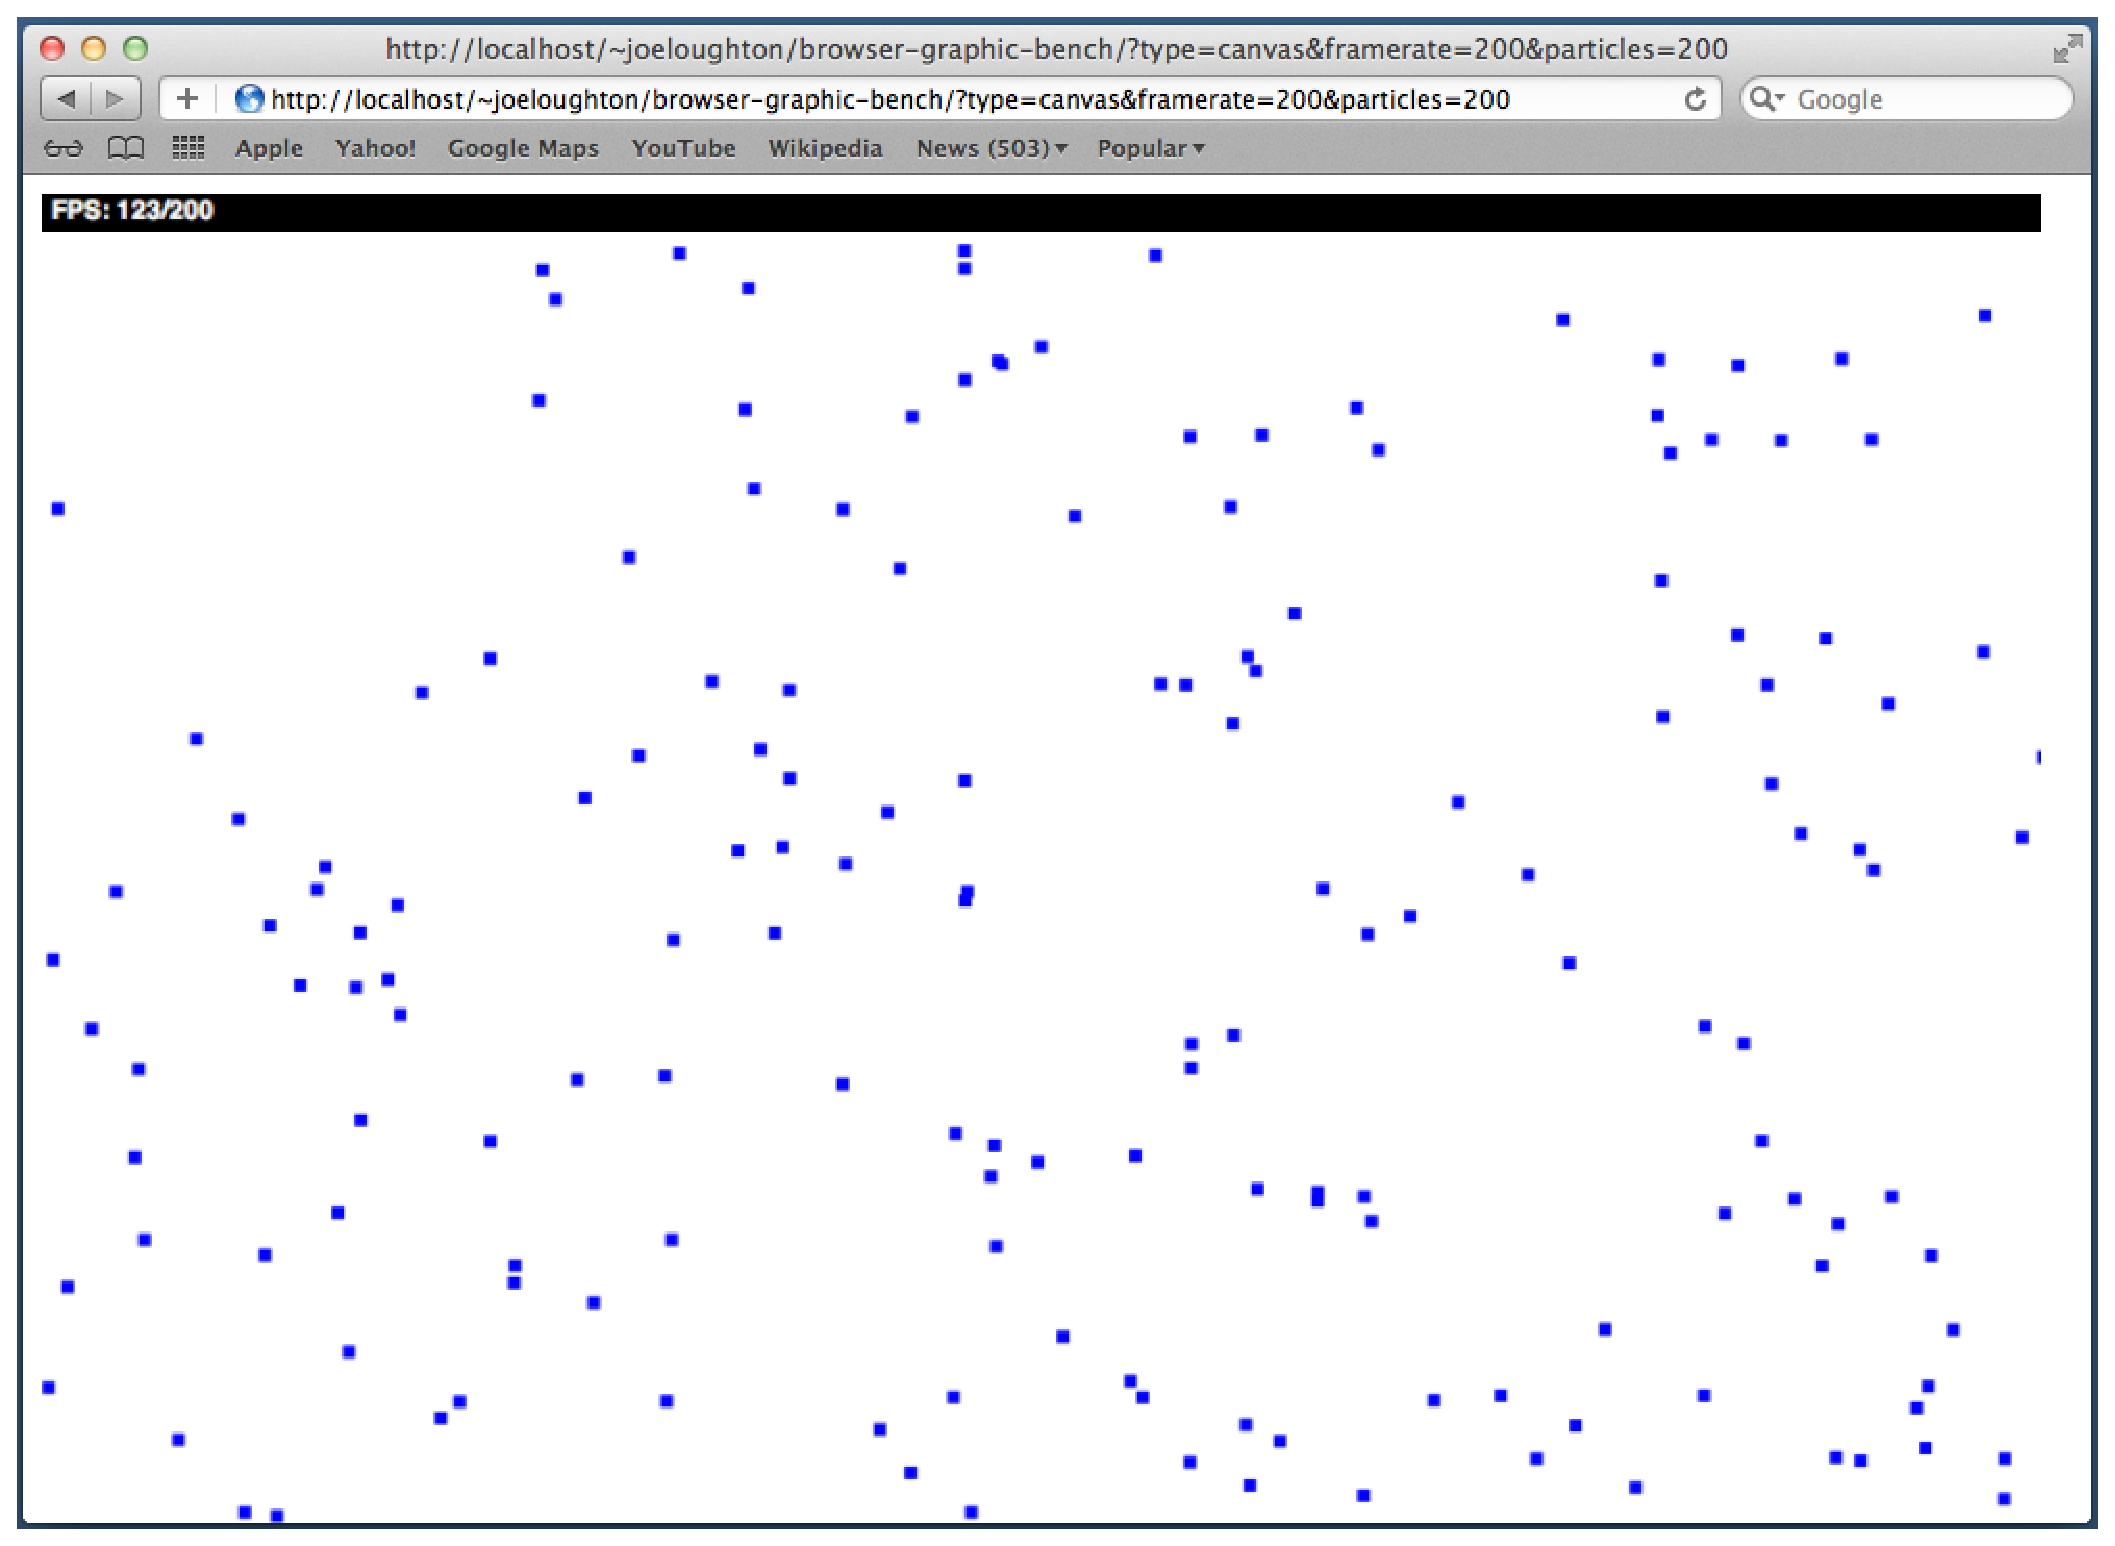
\includegraphics[width=170mm,height=130.08mm]{assets/benchmark-tool.eps}
\caption{}
\label{fig:benchmark-tool}
\end{figure}

\begin{figure}
\centering
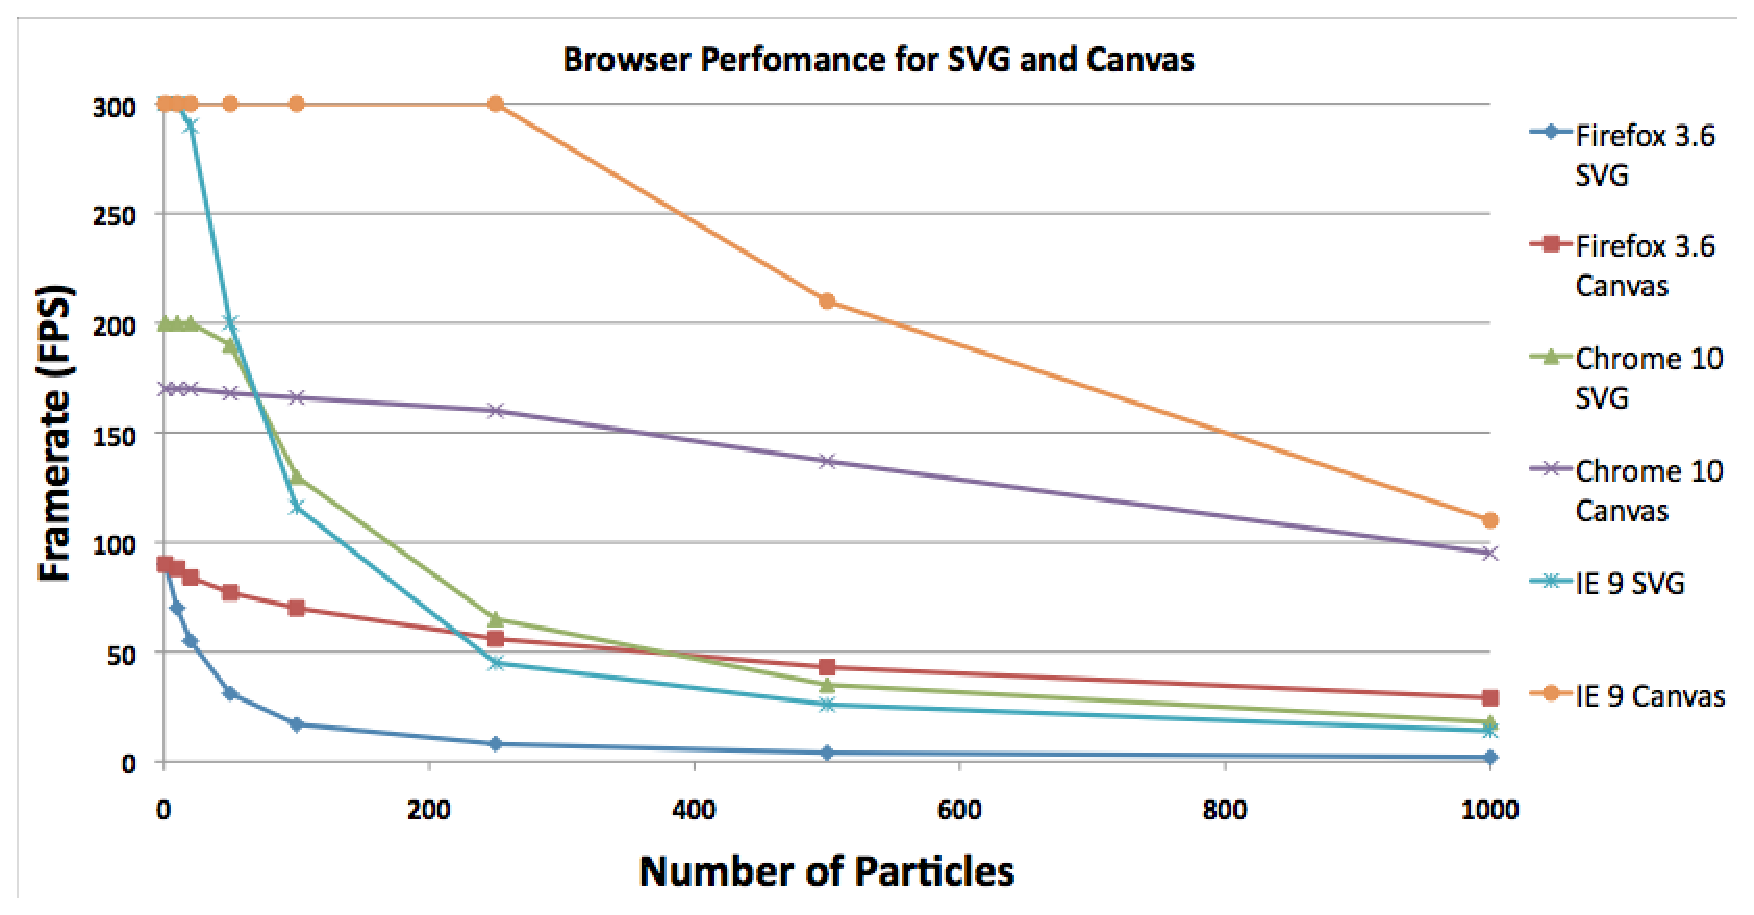
\includegraphics[width=170mm,height=91.67mm]{assets/benchmark-graph.eps}
\caption{}
\label{fig:benchmark-graph}
\end{figure}

\subsection{Libraries}
\label{sec:libraries}
  % Go over the key libraries used
  %   > eg jQuery, Javascript Infovis Toolkit, arbor, QUnit
  % Why did I choose these libraries
  % How did I pick them?

NetMapJs makes use of the jQuery, JavaScript Infovis Toolkit and Abor libraries
in its design. jQuery was used for several reasons \cite{jQuery_website}. Cross
browser support is important such that each user gets the same experience across
different systems.  jQuery functions handles all of this for you an is
especially useful for eliminating browser specific code. jQuery also simplifies
HTML Document manipulation, event handling and AJAX interactions. The JavaScript
Infovis Toolkit provides a framework for producing interactive visualisations
based in the web \cite{thejit_website}. The toolkit includes many very useful
features such as node-edge graph manipulation functions, complex number
arithmetic, animation transitions and so on.

NetMapJs includes a some automatic layout algorithms for initially deciding
where to position nodes in the network map. One of these layouts is a force
directed algorithm.  The Arbor JavaScript library was used for this as it
performs well and provides mechanisms for changing physics parameters such as
gravity and friction \cite{Arbor_website}. The QUnit library is a unit testing
library plug-in for jQuery. This assisted with test driven development during
the implementation stage of the project.


\section{Visual Design} \label{sec:visual-design}
  % Overview of visual design

\subsection{Nodes}
\label{sec:nodes.vis}
  % Design considerations for nodes
  % Nodes can be sub networks
  %   > Helps for scalability
  % Grouping, hiding nodes
  % Combining with symantic zooming
  % Screenshots

  % What are nodes with respect to network maps?
  % What are subnetworks?
  % How have I combined the two?
  % Screenshot 1
  % What is the advantages of this?

Nodes in network maps are traditionally used to express a particular physical or
virtual device. Nodes are joined together by edges which represent the
relationship between then. Subnetworks are a specific group of devices that
relate to each other in some way. Subnetworks networks may be made up of other
subnetworks and altogether they can be seen as a single network. It is possible
to apply this concept to nodes when designing a visualisation. Nodes can
visually contain sub nodes and so on for a given number of depth levels. Nodes
that fall into this category will be referred to as group nodes.

Figure \ref{fig:nodes1.0} shows the Hamilton (HLZ) PoP for the Karen network.
The outer circle marks the HLZ node and the smaller, solid circles inside
illustrate the sub nodes of that PoP. This grouped effect causes the viewer the
assume that the sub nodes are related to each other through a common parent
node. Figure \ref{fig:nodes1.1} shows a more zoomed in view of the same HLZ
group node. The parent node and edges are now faded out so the focus is now on
the sub nodes and edges. This idea of zooming and adding detail is explained in
Section \ref{sec:navigation.vis}. There needs to be way of laying out the sub node
within a group. Different group nodes may make sense to be laid out differently.
The HLZ group node is using a star layout. Layout considerations are discussed
in Section \ref{sec:layouts.vis}.

  % May want to see nodes only at a given level...
  % How have I done this?
 
\begin{figure}
\centering
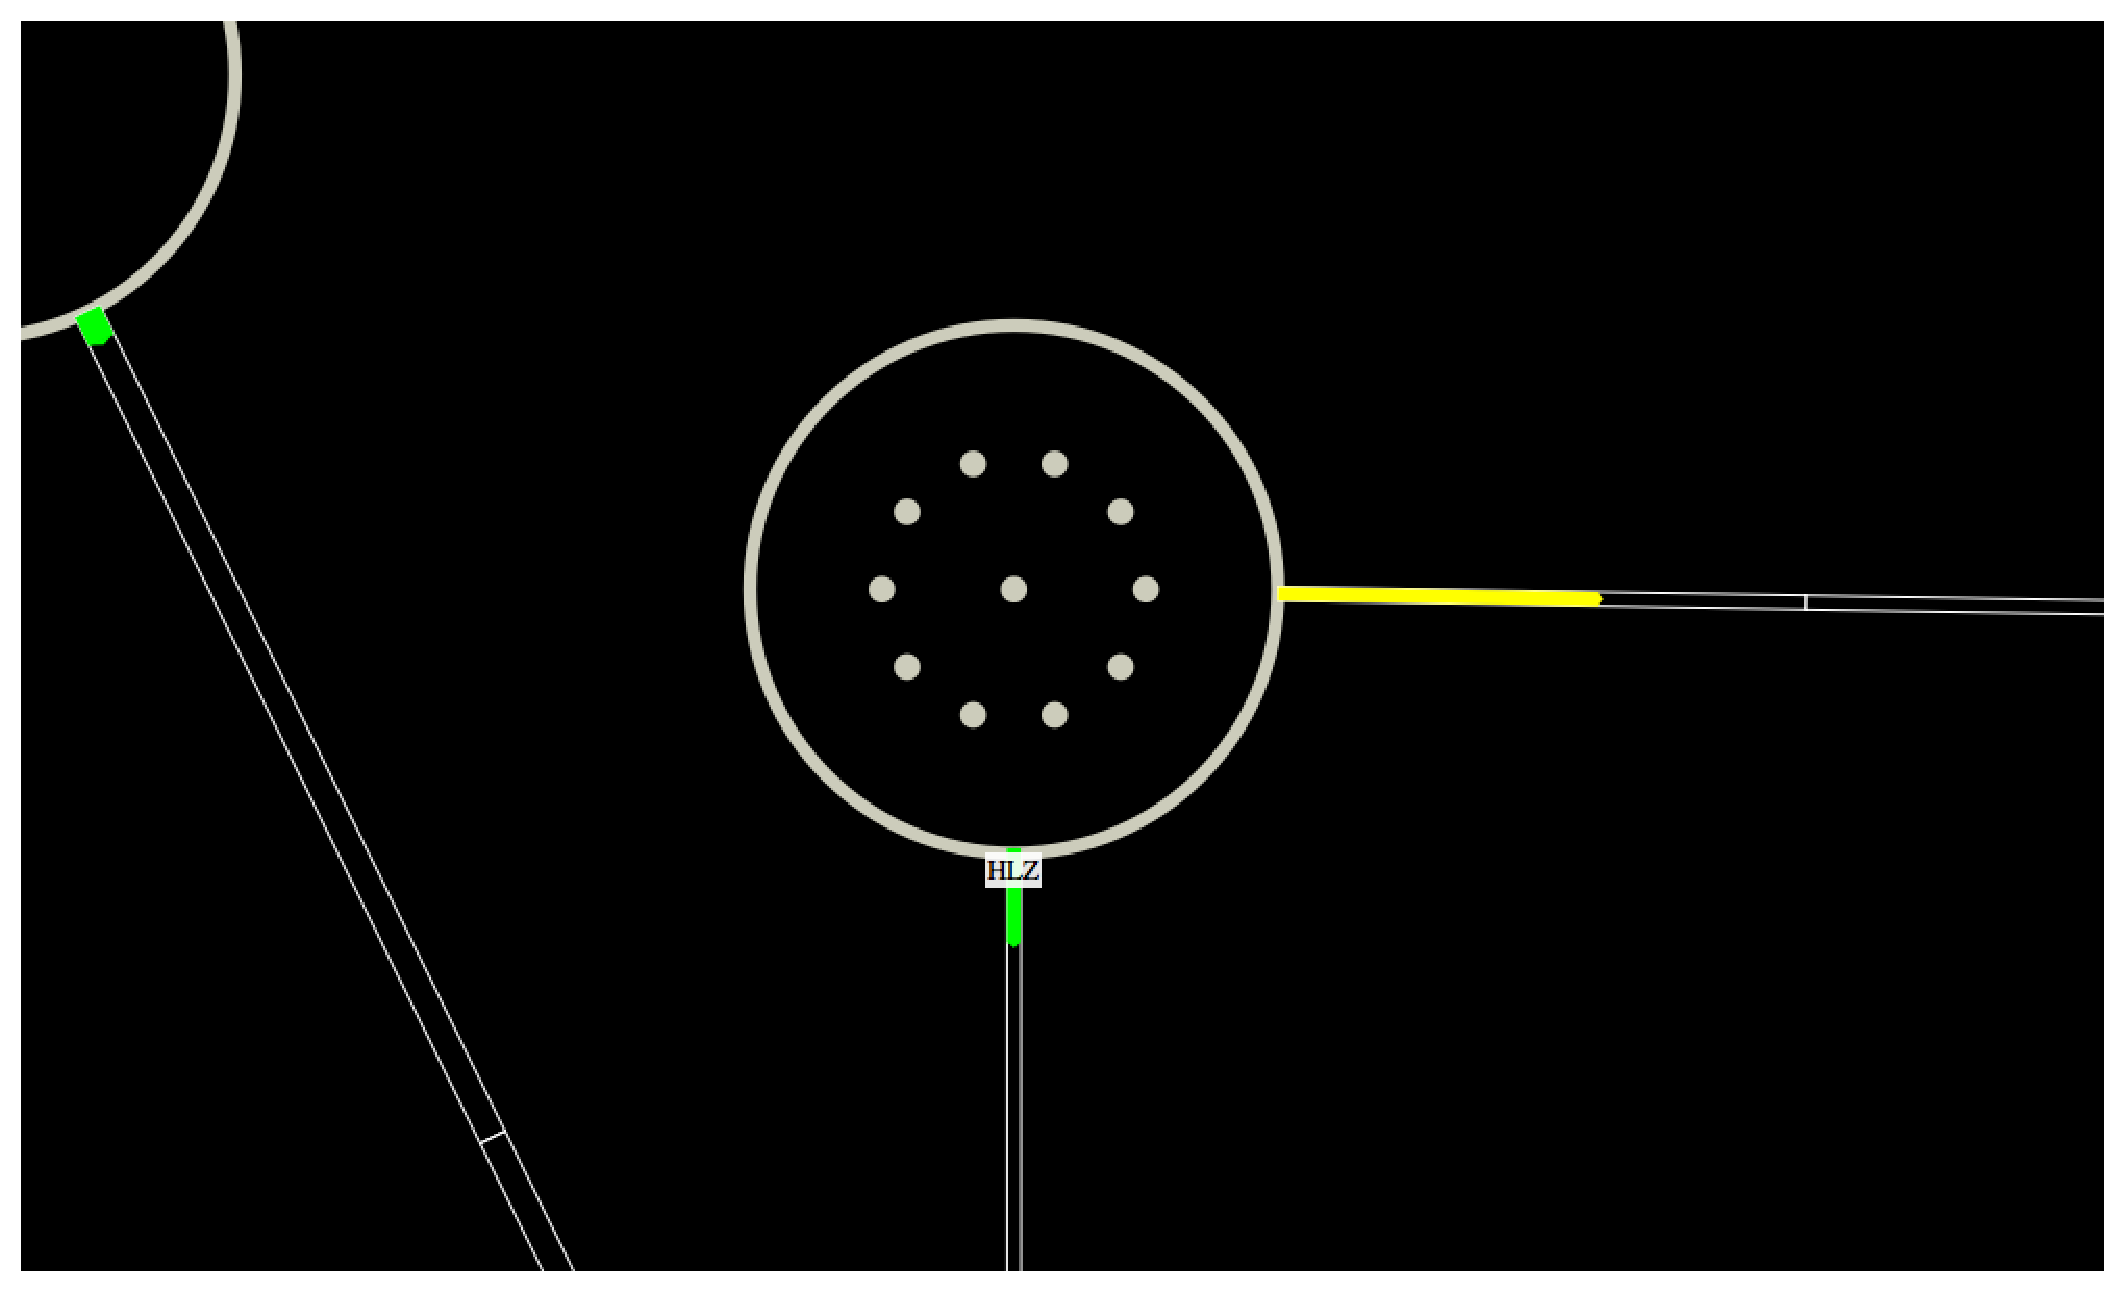
\includegraphics[width=170mm,height=107.58mm]{assets/nodes1-0.eps}
\caption{}
\label{fig:nodes1.0}
\end{figure}

\begin{figure}
\centering
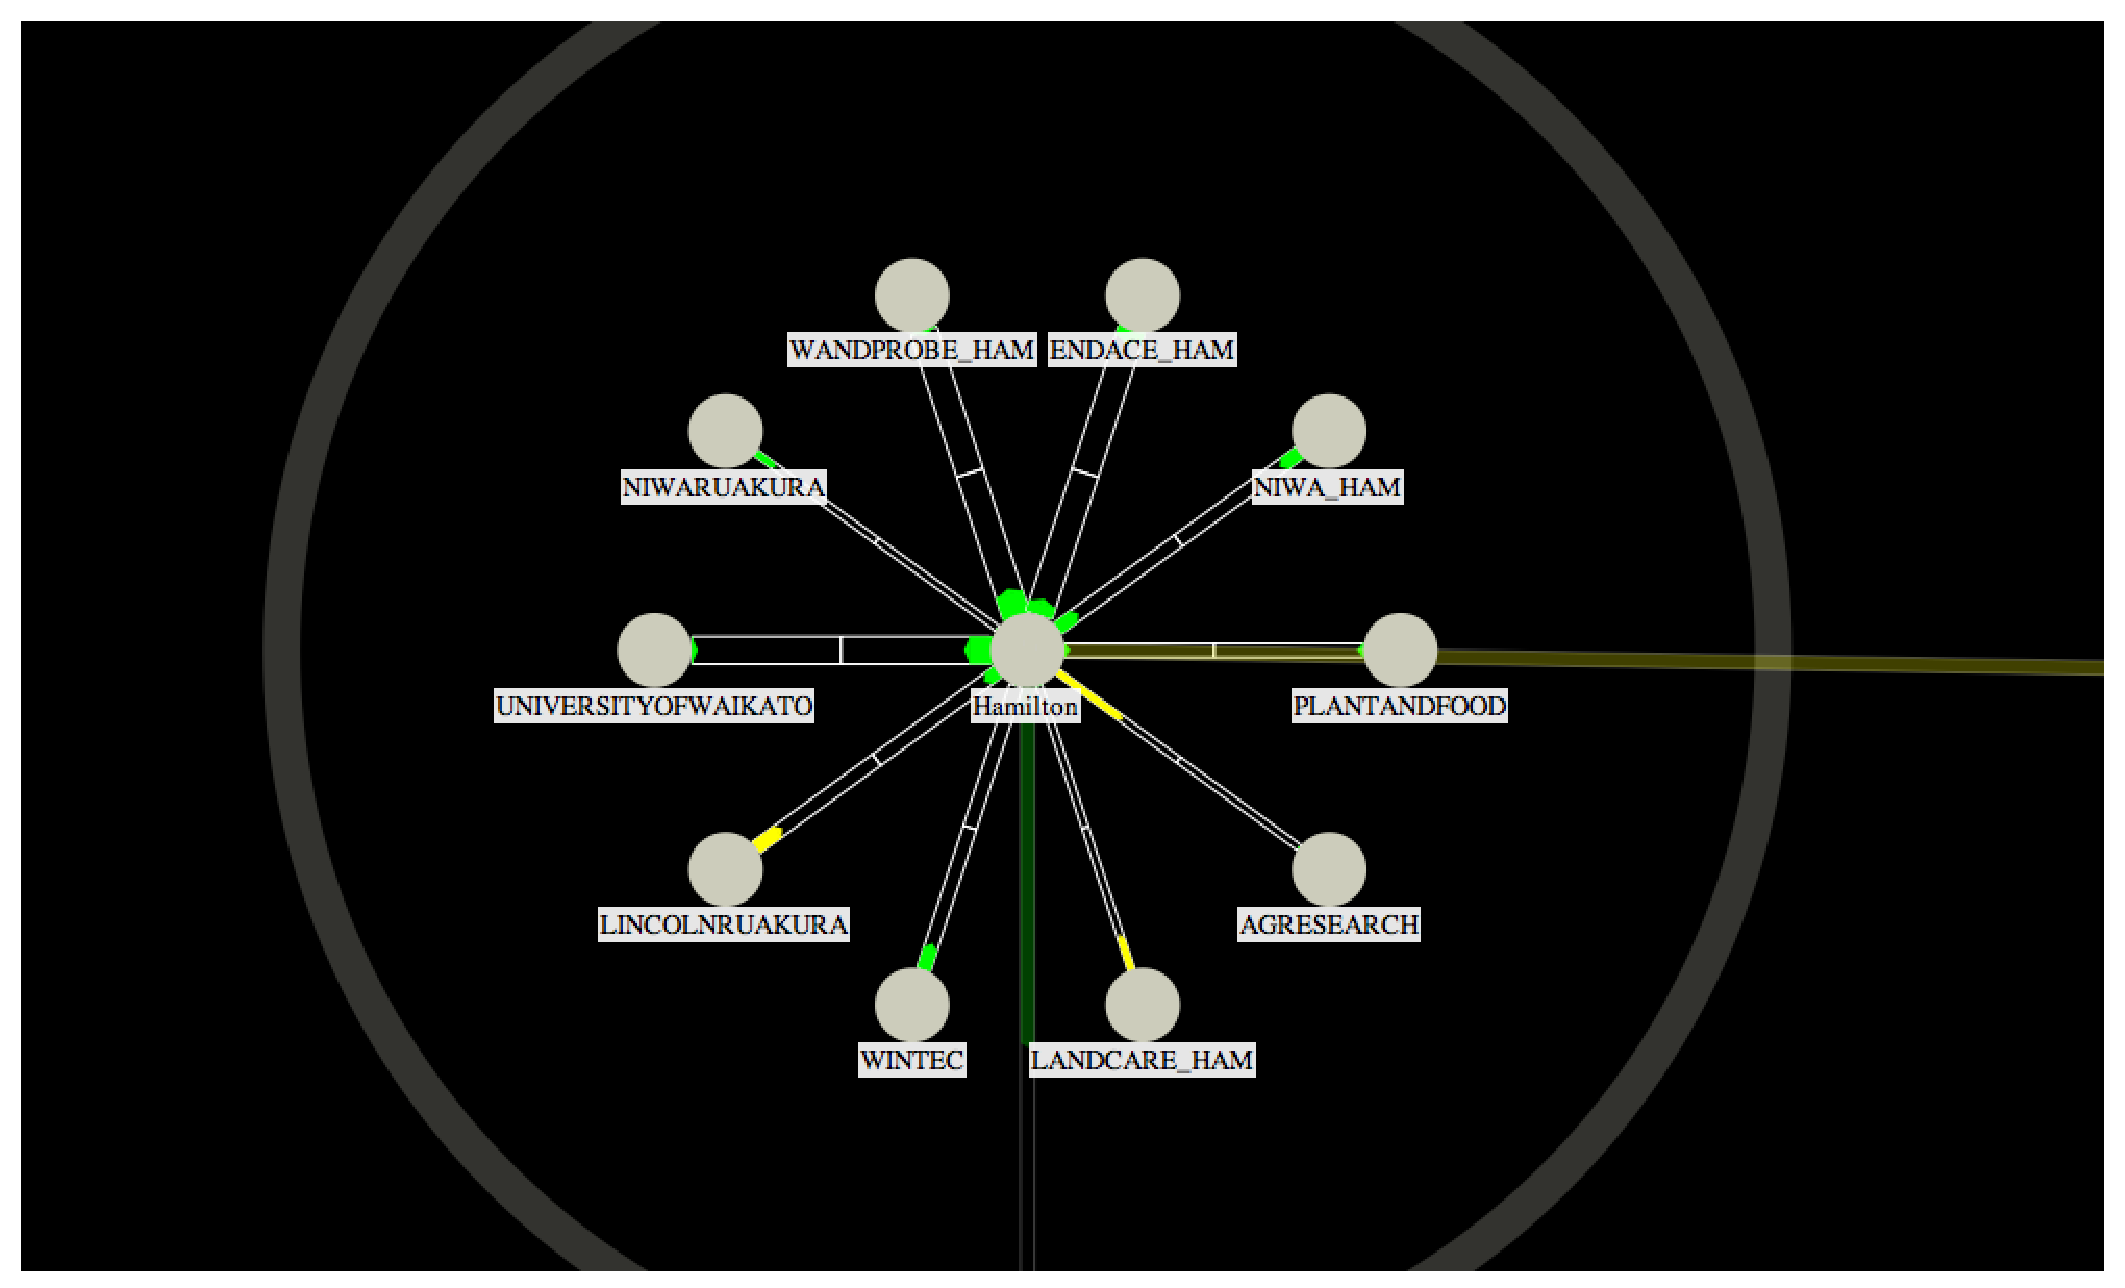
\includegraphics[width=170mm,height=101.93mm]{assets/nodes1-1.eps}
\caption{}
\label{fig:nodes1.1}
\end{figure}

\subsection{Edges}
\label{sec:edges.vis}
  % Simple line between two nodes
  % Can make use of this space more effectively
  % Explain the visual design of my way
  %   > visualisation principles included
  %   > Quantitative vs qualitative
  % Screenshots

Edges between nodes in a network map indicate that two or more devices are
connected to each other by some medium. A single line between two nodes is
enough to show this relationship. If this line is thin then it reduces the
amount of clutter for the same number of edges \cite{Tufte_2001}. Figure
\ref{fig:edges1.0} shows the display of a network with many nodes, displayed in
a clear way.
% TODO: fill out paragraph more?

In the case of network maps, there is often monitoring data available that
directly relates to the performance of a given edge medium. This data could be
accessed through a separate view in the visualisation but there are advantages
to showing this directly on map. For example, if something goes wrong with a
link then an indication on the main view on the visualisation will attract the
users attention immediately opposed to if the user had to follow some
interaction sequence to get at the data. For his project a new way of
visualising quantitative variables describing a bidirectional network connection
was developed. In particular, variables which have some sort of limit such as
the bandwidth or packet loss of a link.

Figure \ref{fig:edges1.1} gives an overview of how the connection visualisation
works by using bandwidth as an example. A rectangle is drawn between two nodes
and split into two at the mid point. The side of the split rectangle closest to
a given node represents the direction from that node to the destination. The
height of each of the rectangular sections indicates the total quantity of the
variable. For bandwidth, this would be the total for that direction of the link
and may be different to the other direction in the case of asymmetric
connections. Arrows extend from a given node towards another with the length
being relative to the percentage of the variable's proximity to its upper limit.
The colour of the arrow is defines some user defined categorical variable such
as the health of the network link.

The design for this graphic took careful consideration of information
visualisation principles. Position and length are the most accurate methods for
encoding quantitative variables \cite{Spence_2007}. The design uses length to
show total and percentage utilisation. The use of position is also shown in the
arrow as a proportion of the total rectangular section. Colour hue is effective
at displaying categorical variables which is how it is being used in the
visualisation. Figure \ref{fig:edges1.2} shows this design implemented in
NetMapJs and is being used to show that bandwidth between the Palmerston North
and Wellington PoPs in the Karen map.

\begin{figure}
\centering
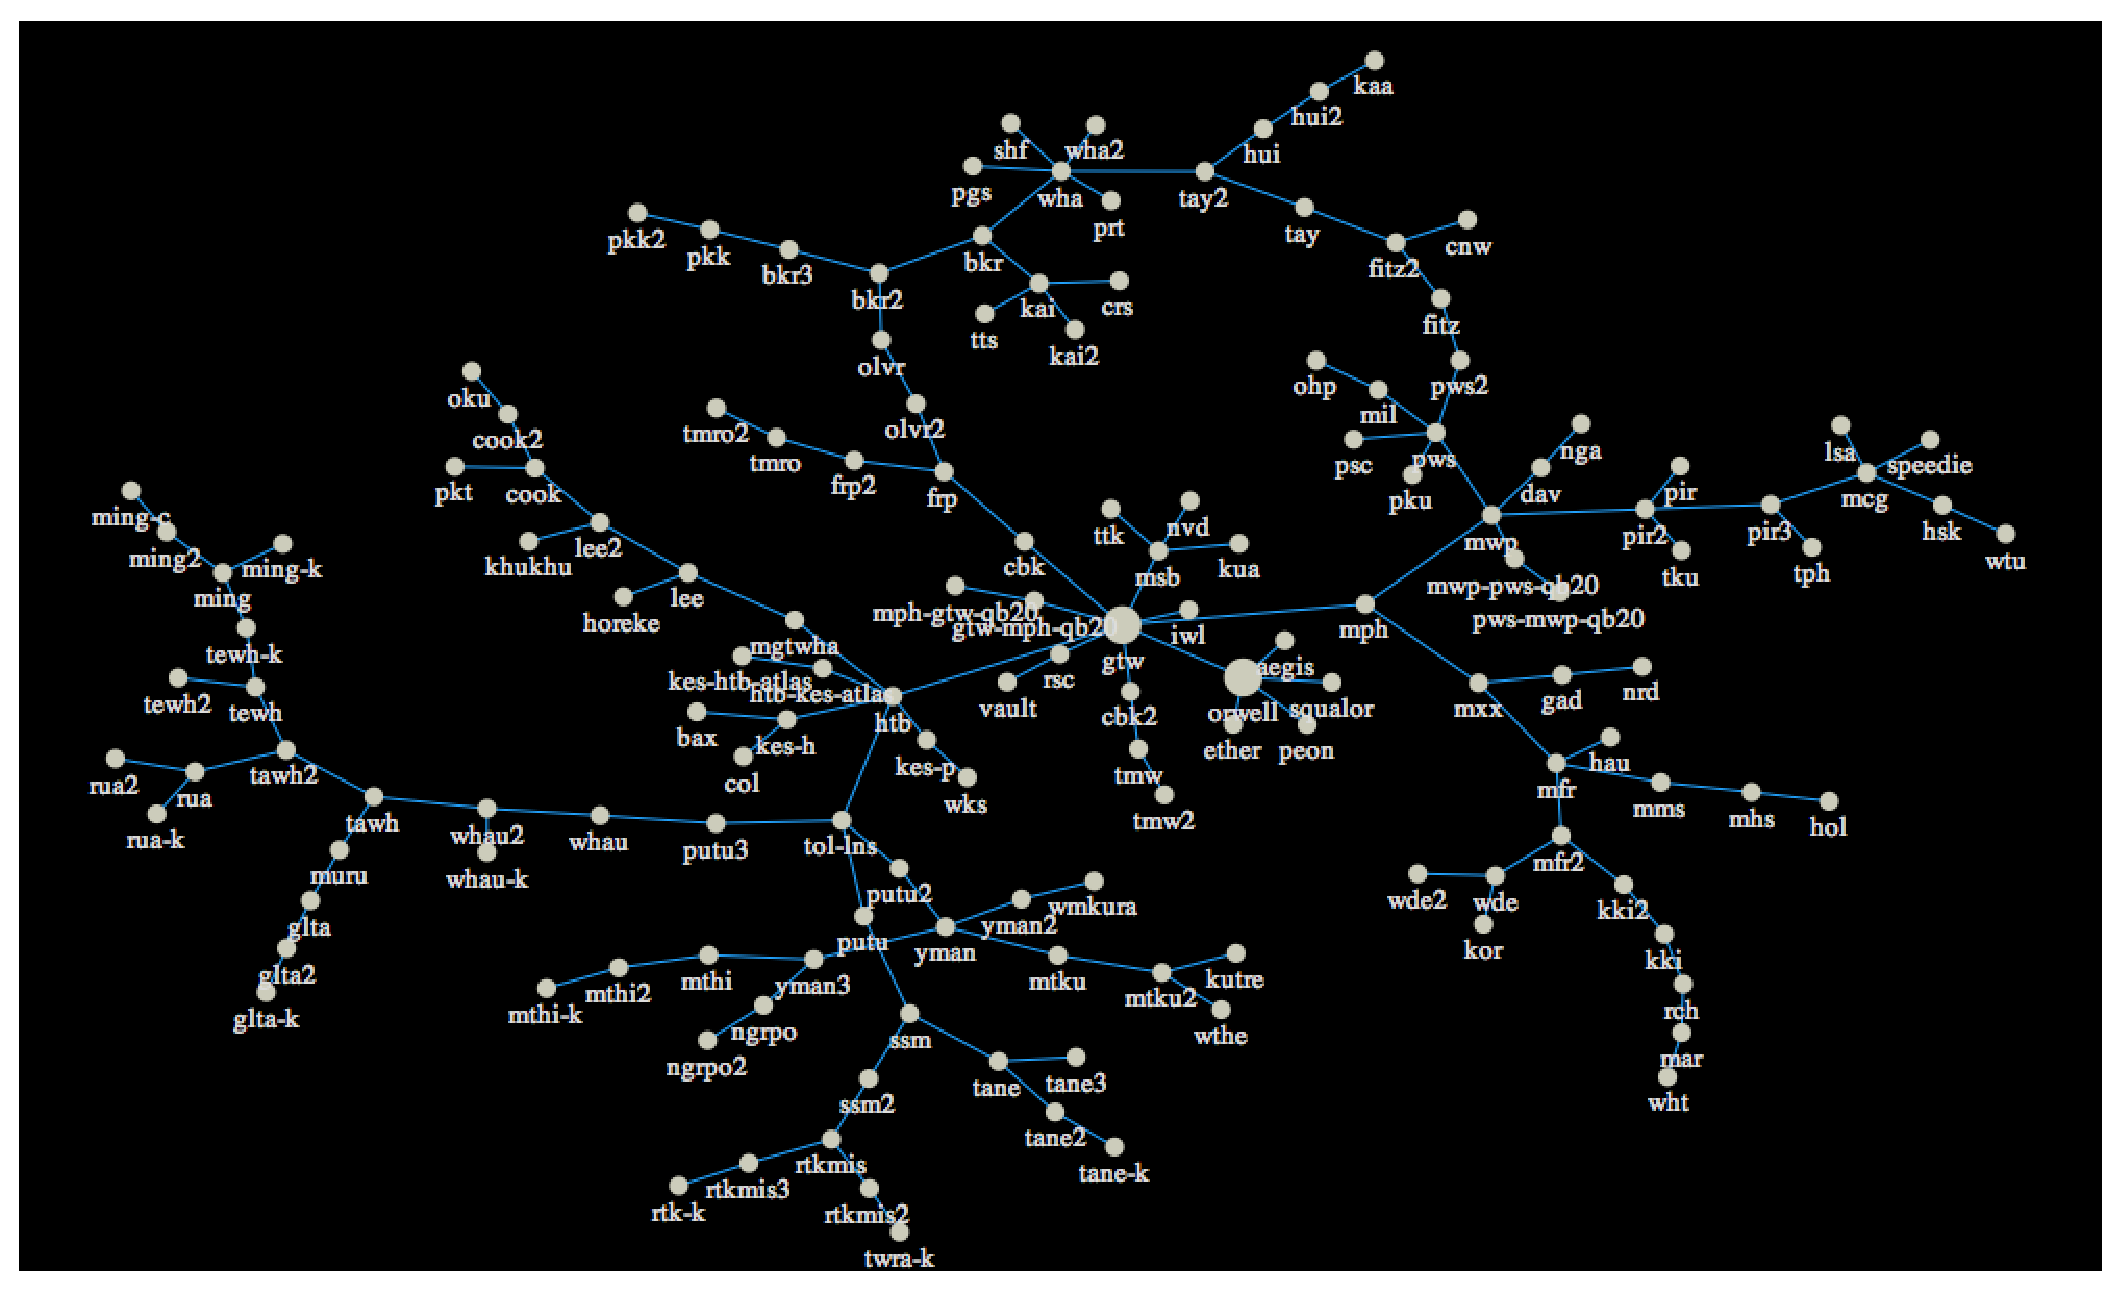
\includegraphics[width=170mm,height=102.54mm]{assets/edges1-0.eps}
\caption{}
\label{fig:edges1.0}
\end{figure}

\begin{figure}
\centering
\includegraphics[width=170mm,height=59.03mm]{assets/edges1-1.eps}
\caption{}
\label{fig:edges1.1}
\end{figure}

\begin{figure}
\centering
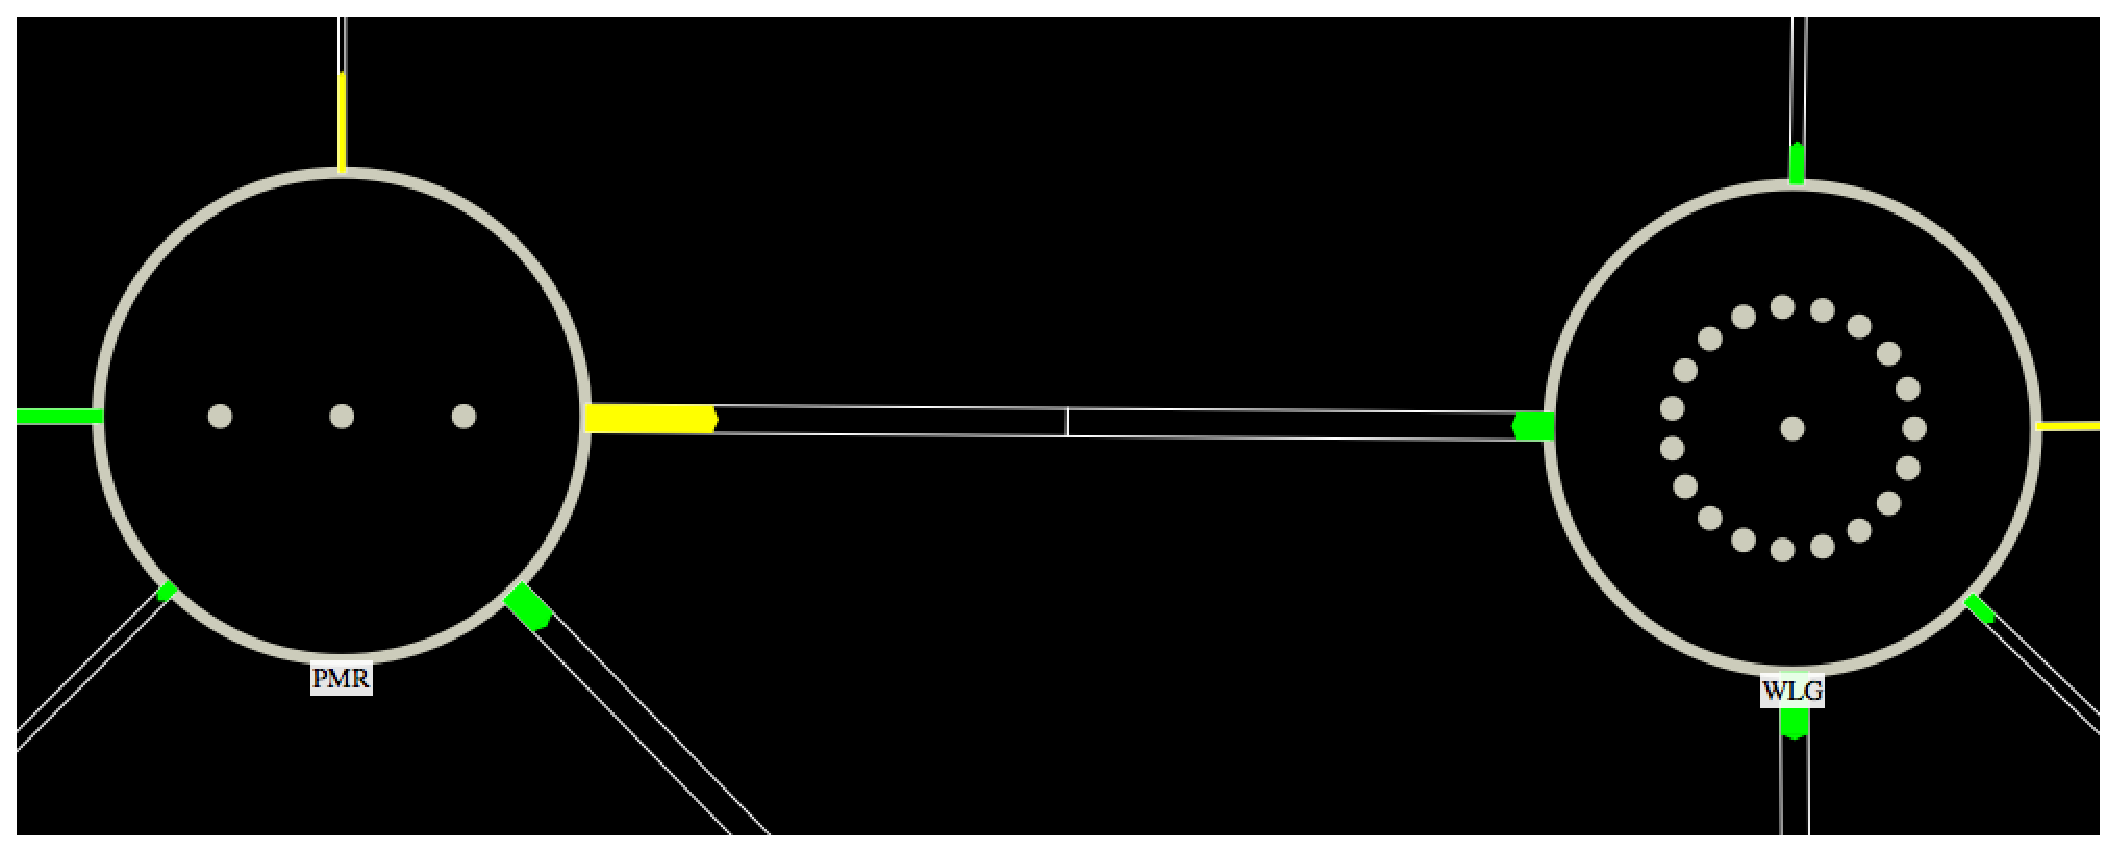
\includegraphics[width=170mm,height=70.21mm]{assets/edges1-2.eps}
\caption{}
\label{fig:edges1.2}
\end{figure}

\subsection{Layouts}
\label{sec:layouts.vis}
  % Explain importance of node layout
  %   > Different subgroups - different layouts
  %       - reference Java3D paper - has lots of layout talk
  %   > Groups have layouts
  % Which layouts did I implement and why
  % Screenshots

% importance
%   > Too much time required to statically layout large networks
%   > Need to minimise overlapping
%   > Need to maximise user understanding and recognition
%   > Good layout can lead to greater understanding where as bad can be
%   missleading
% “Finding the Best Viewpoints for Three–Dimensional Graph Drawings
% 

% Herman_1998 - great graph layout issues as well as focus, context techniques
% and zoom//pan issues.
% Graph Visualization and Navigation in Information Visualization
% 

A good layout of nodes in a network map is important to maximise the insigt and
undestanding possible to the user. A bad layout can lead to cluttering of nodes
and edges or worse, a misunderstanding of the underlying data. The use of 3D
layouts effectively give more available space for positioning nodes but can
introduce new problems. Nodes and edges in a 3D layout may occlude other objects
and it is hard to choose an ideal perspective within the 3D
space \cite{Eades_1998}. 2D layouts are used in this project which simplifies the
use of semantic zooming as described in Section \ref{sec:navigation.vis}. 

Two basic 2D layout algorithms were used in this project in addition to
statically defining node positions. A force directed and star algorithm. These
two were chosen because they were known to work well with the example datasets
and provide a good starting point over just static layouts. A complete network
map tool would include many more layout algorithms to cope with a wider range of
network layout structures \cite{Paul_2000}. Figure \ref{fig:edges1.0} shows
Rural Link's network laid out using the force directed algorithm. The algorithm
lays out the network particularly well due to its tree like structure. In
particular, there are no overlapping edges or nodes in the map. Redundant
connections are shown clearly by branches that join up to form a loop. 

Sub groups may make sense to have separate layout algorithm applied to them when
the underlying network structures are different. An example of this is
demonstrated in Figure \ref{fig:layouts1.1}. The overall view of the Karen map
contains statically defined node positions that are based of layout designs by a
graphic designer. When the user zooms in to a particular PoP, it can be seen
that the layout of that group is a star layout. One central node, the
distribution router, connects to all the other devices in that PoP.

\begin{figure}
\centering
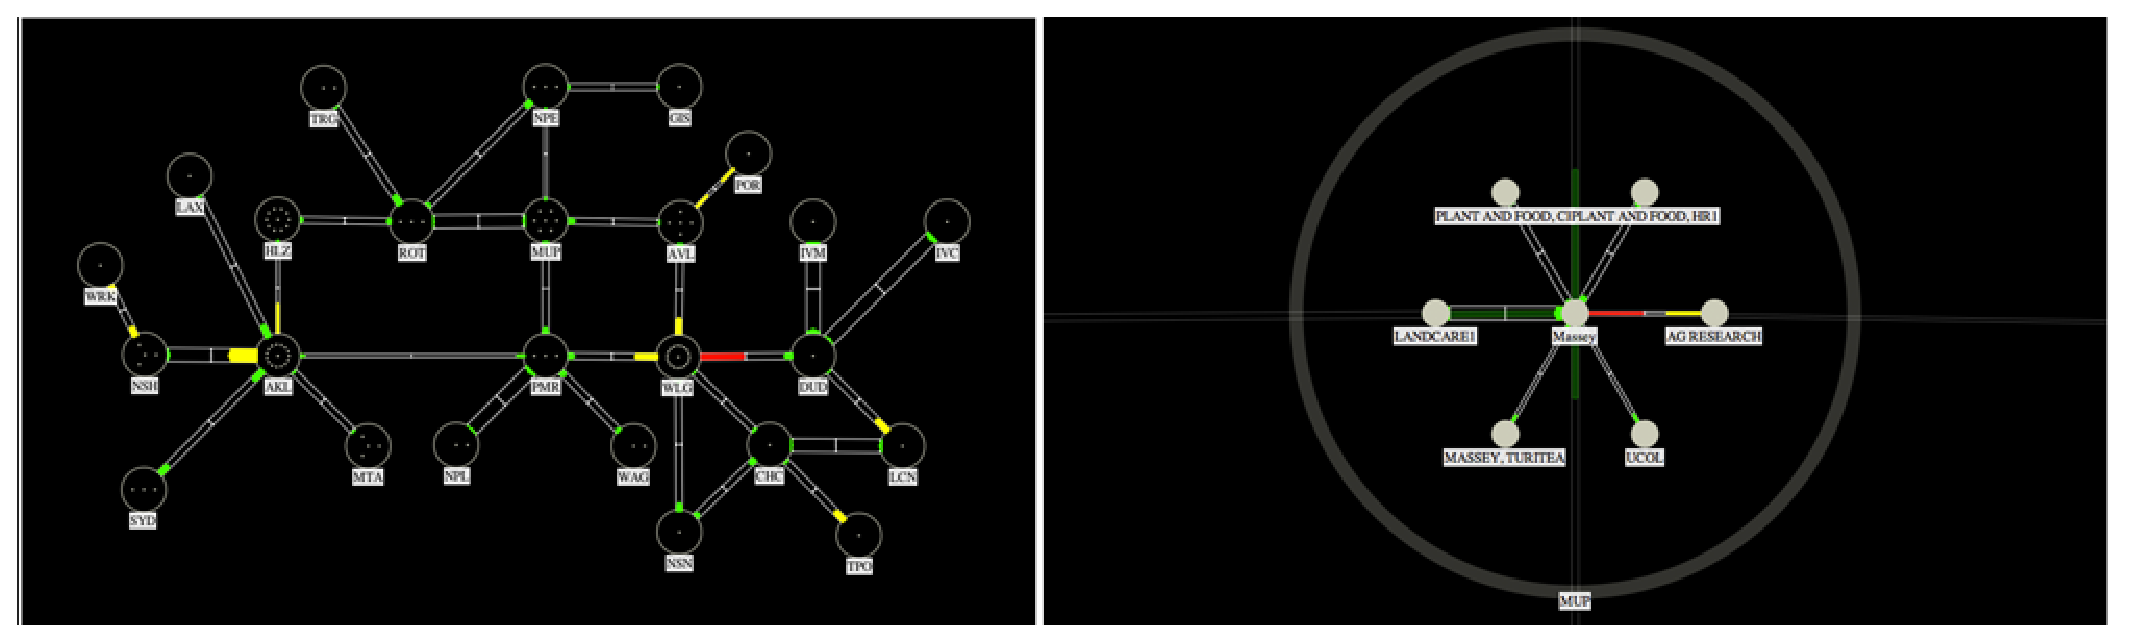
\includegraphics[width=170mm,height=49.34mm]{assets/layouts1-1.eps}
\caption{}
\label{fig:layouts1.1}
\end{figure}


\subsection{Navigation}
\label{sec:navigation.vis}
  % Details of navigation
  % Why is getting it right important
  % Issues relating to navigation
  % Zoom, pan, zoom/center nodes, follow edges
  % Screenshots

Layout algorithms can be good at laying out large graphs properly but there is a
limit to their effectiveness. At some level of network size or density the
limits of these algorithms will be reached and ideal layouts will no longer be
guaranteed. It is also likely that a user can not even decipher information and
patterns from such large networks. It is therefore useful to combine layout
algorithms with other techniques in order to remain scalable \cite{Herman_1998}.
Grouping devices into subnetworks is a reduction technique as described in
Section \ref{sec:nodes.vis}. 

Another technique for reducing networks is semantic zooming \cite{Perlin_1993}.
This is different from geometric zooming in that changes are made to the level
of information displayed while moving towards a specific area of a graph. What
would perhaps be visually overwhelming if presented all at once, can instead be
trickled out to the user as they indicate that they are more interested in a
particular subsection of a network. NetMapJs uses this type of zooming along
with panning to effectively navigate throughout large networks. 

Figure \ref{fig:nav1.0} shows more detail being revealed to the user as they
zoom in to a sub group of the Karen network. In the fully zoomed out view it is
important to indicate that there is distant content so that the user is aware
that they can zoom in for further detail \cite{Spence_2007}. Sub groups indicate
that they contain more detail by using small dots and as the user zooms in to
that group, more detail such as labels and edges between nodes appear. At this
point, the group node graphic and its external edges become faded out which
allows the user to focus more on the current groups detail while still being
aware of what group the nodes are apart of.

While implementing the design of NetMapJs it became apparent that it got
increasingly difficult to navigate between nodes in the map as you zoomed deeper
into sub groups. For example, when zoomed into the Hamilton PoP in the Karen
map, it would require a lot of user interaction to view the directly connected
Auckland PoP. Several drags of the mouse would be required to pan towards
Auckland or zooming back out and in again even made sense. To eliminate this
problem, two navigation features were added.

The first feature enables the user to follow an edge to the node on the other
end of it in one click. For example, if the user is currently zoomed in to the
Hamilton PoP and wants to go to the Auckland PoP, they must simply click the
edge that connects the two. An event triggered tooltip is displayed over an edge
to notify the user of what node lies on the other end of it. This is shown in
Figure \ref{fig:nav1.1}. The addition of animated transitions between view
changes allow users to keep context and to absorb the change
\cite{Lamping_1995}.  NetMapJs uses animation this way to transport the user to
the new view such that they get an sense of where in the network they are moving
to. A direct jump from the source to destination node, risks confusing their
perceived location in the overall network.

The other feature for improving navigation is zooming and centering nodes. When
a user knows that they want to view a particular group node normally they would
perform a sequence of zooming and panning actions to bring it into focus. This
feature allows the user to simply right click on a group node to automatically
bring it into focus again using animation to change the views. Figure
\ref{fig:nav1.2} demonstrates this effect. Combining these two features actually
makes zooming and panning not necessary. The user is able to freely move around
the network map quickly and effectively. The manual controls are still useful to
make minor adjustments to the view and to zoom back out.

\begin{figure}
\centering
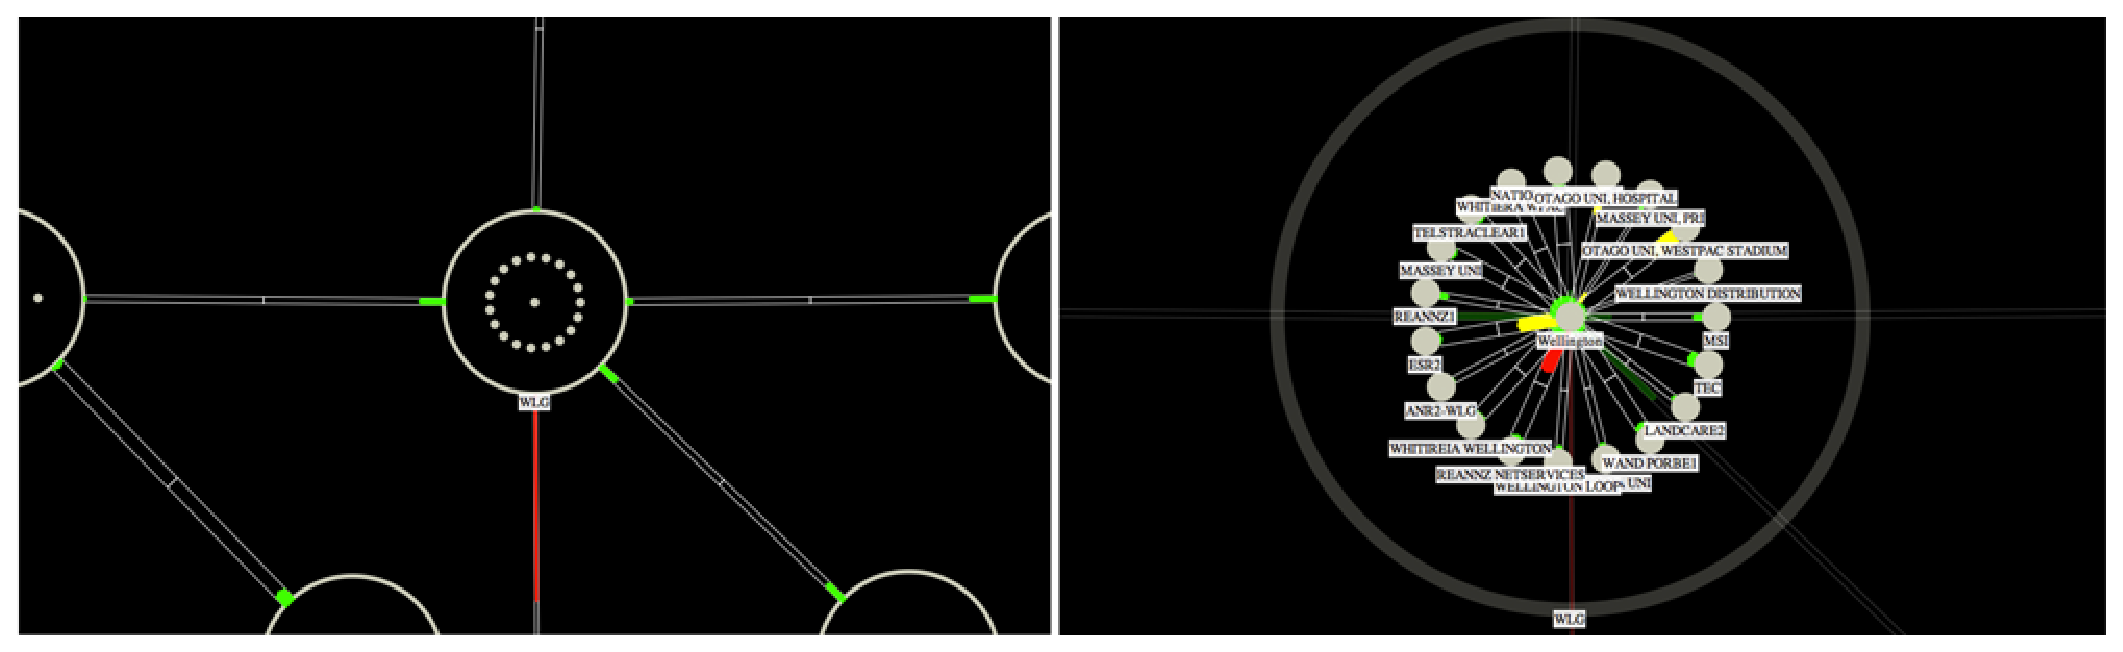
\includegraphics[width=170mm,height=53mm]{assets/nav1-0.eps}
\caption{}
\label{fig:nav1.0}
\end{figure}

\begin{figure}
\centering
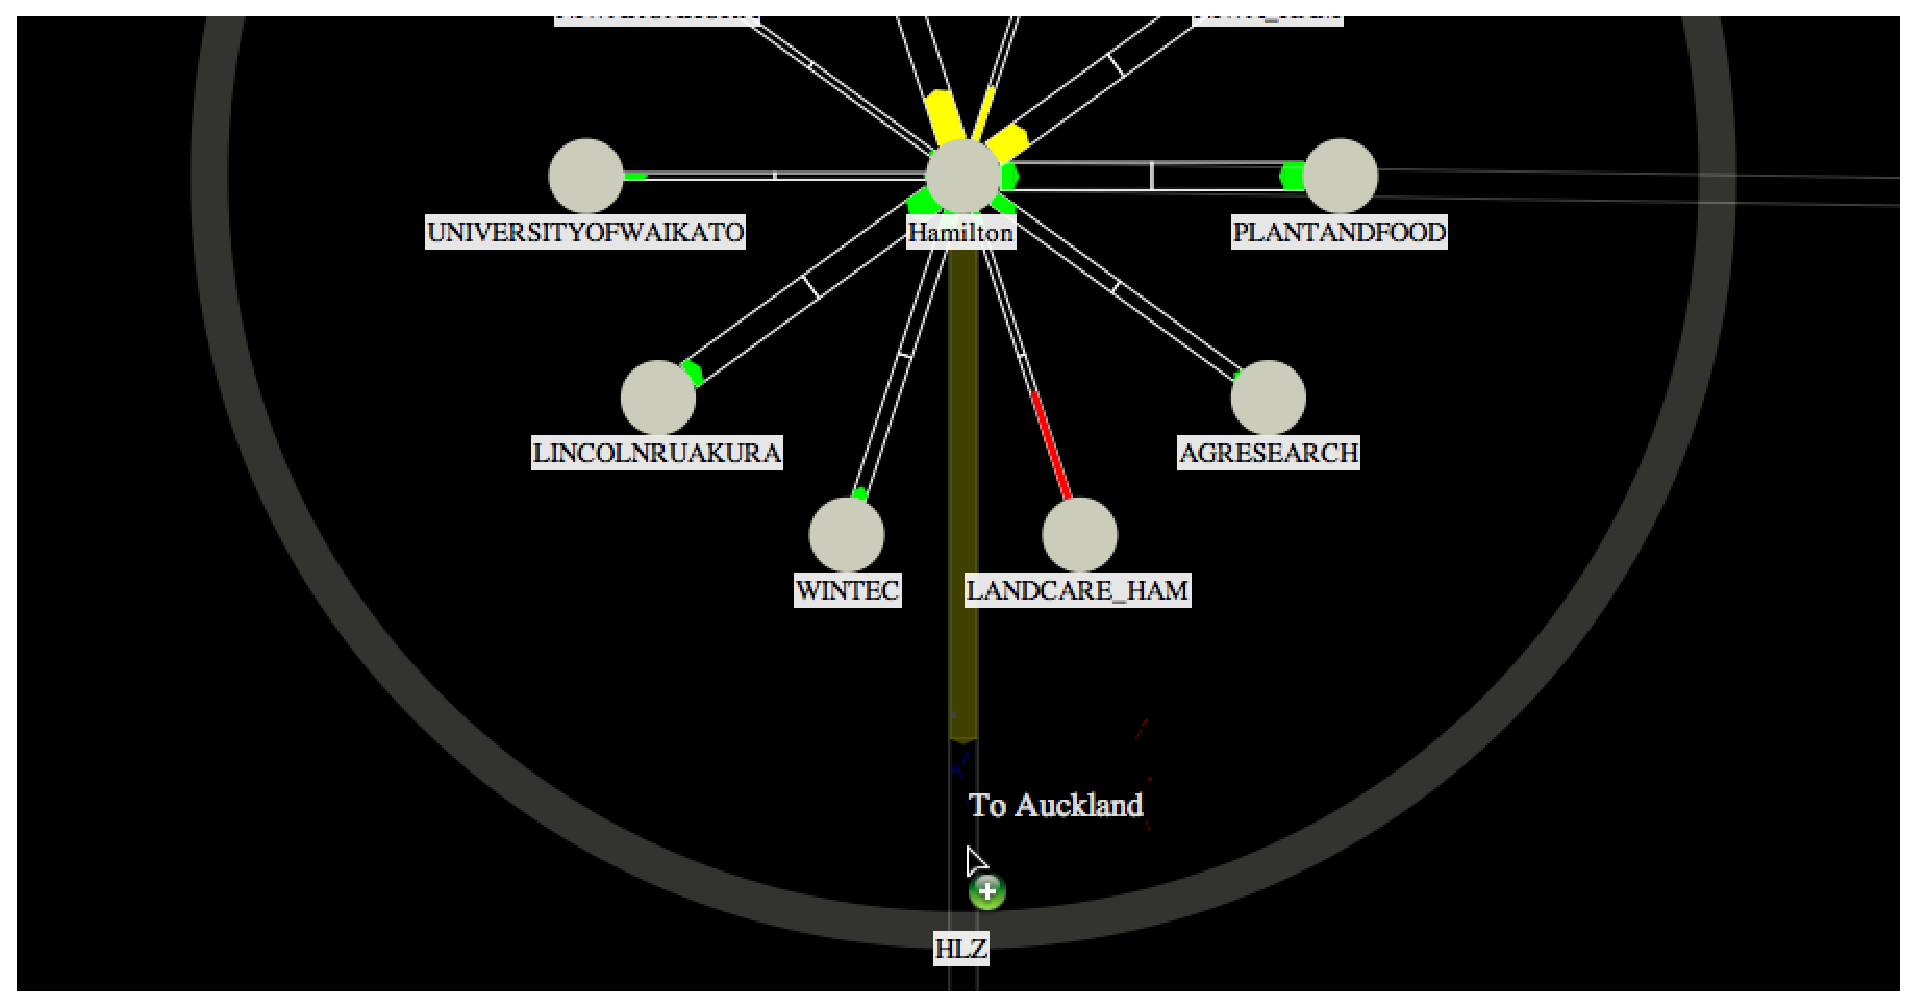
\includegraphics[width=170mm,height=88.01mm]{assets/nav1-1.eps}
\caption{}
\label{fig:nav1.1}
\end{figure}

\begin{figure}
\centering
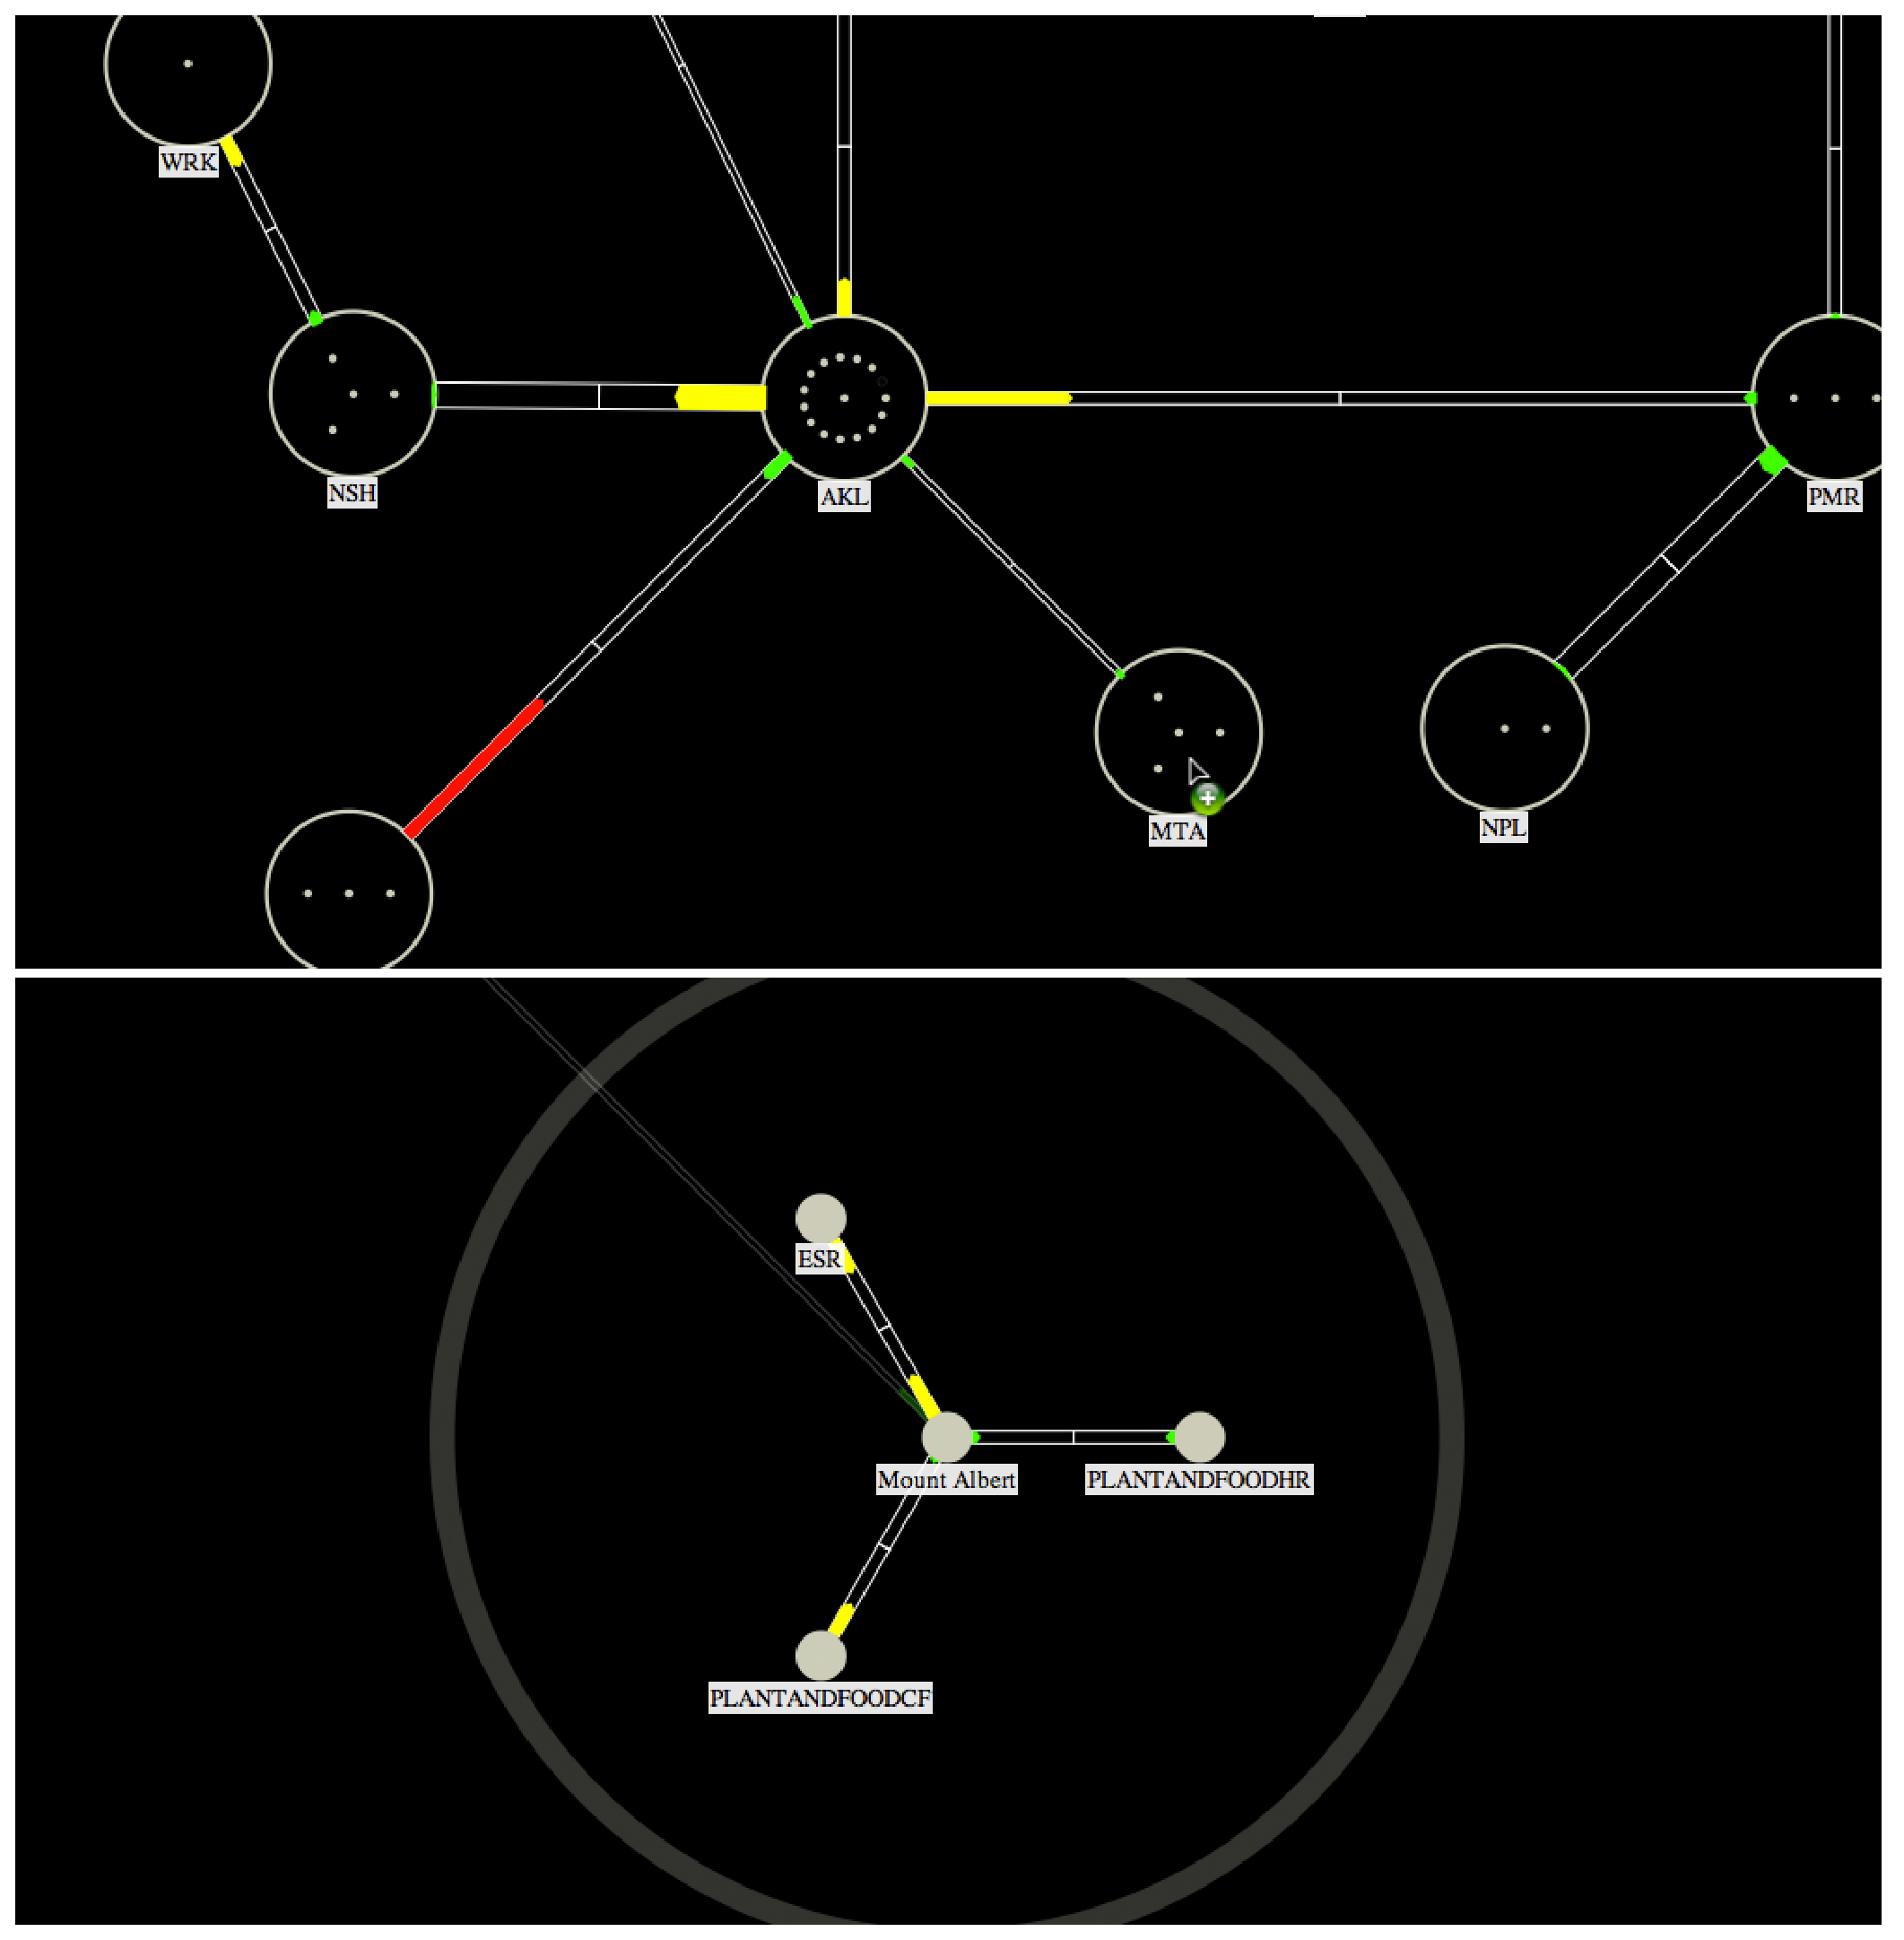
\includegraphics[width=170mm,height=173.22mm]{assets/nav1-2.eps}
\caption{}
\label{fig:nav1.2}
\end{figure}

\subsection{Overviews}
\label{sec:overviews.vis}
  % The problem - 
  % How is it solved - 
  % What does it look like - 
  %   > 

As a user zooms in to deeper levels of the network map it becomes easy for them
lose context about where in the overall network they are. It is not preferred
for the user to have to zoom out just to regain this context. To address this,
NetMapJs makes use of multiple overview maps that each display a particular
level of the network. Where a level refers to a zoom range in which no detail is
added or removed. Starting from an initial zoomed out view, as the user zooms
in to a sub group of the network, a separate overview map for that level is
added to a stack of overviews. As the view port gets deeper into the map, more
and more overviews are added in to this stack. When the user zooms back out, the
reverse happens and overviews are removed from the stack.

Figure \ref{fig:overviews1.0} demonstrates this stacking effect. Also visible in
the screen shot, is yellow rectangles that have a cross-hair intersecting the
middle. The outline of the rectangles show were exactly the user's view port is
situated in the map as a whole as well as in each individual level. A cross-hair
was used to make sure the view port location can still be identified on higher
levels in which the rectangle becomes too small to see. The overviews are also
linked to the main visualisation such that the user can click and drag the
rectangles to move the main view port accordingly. This allows for large
movements across the map while in a zoomed in view.

\begin{figure}
\centering
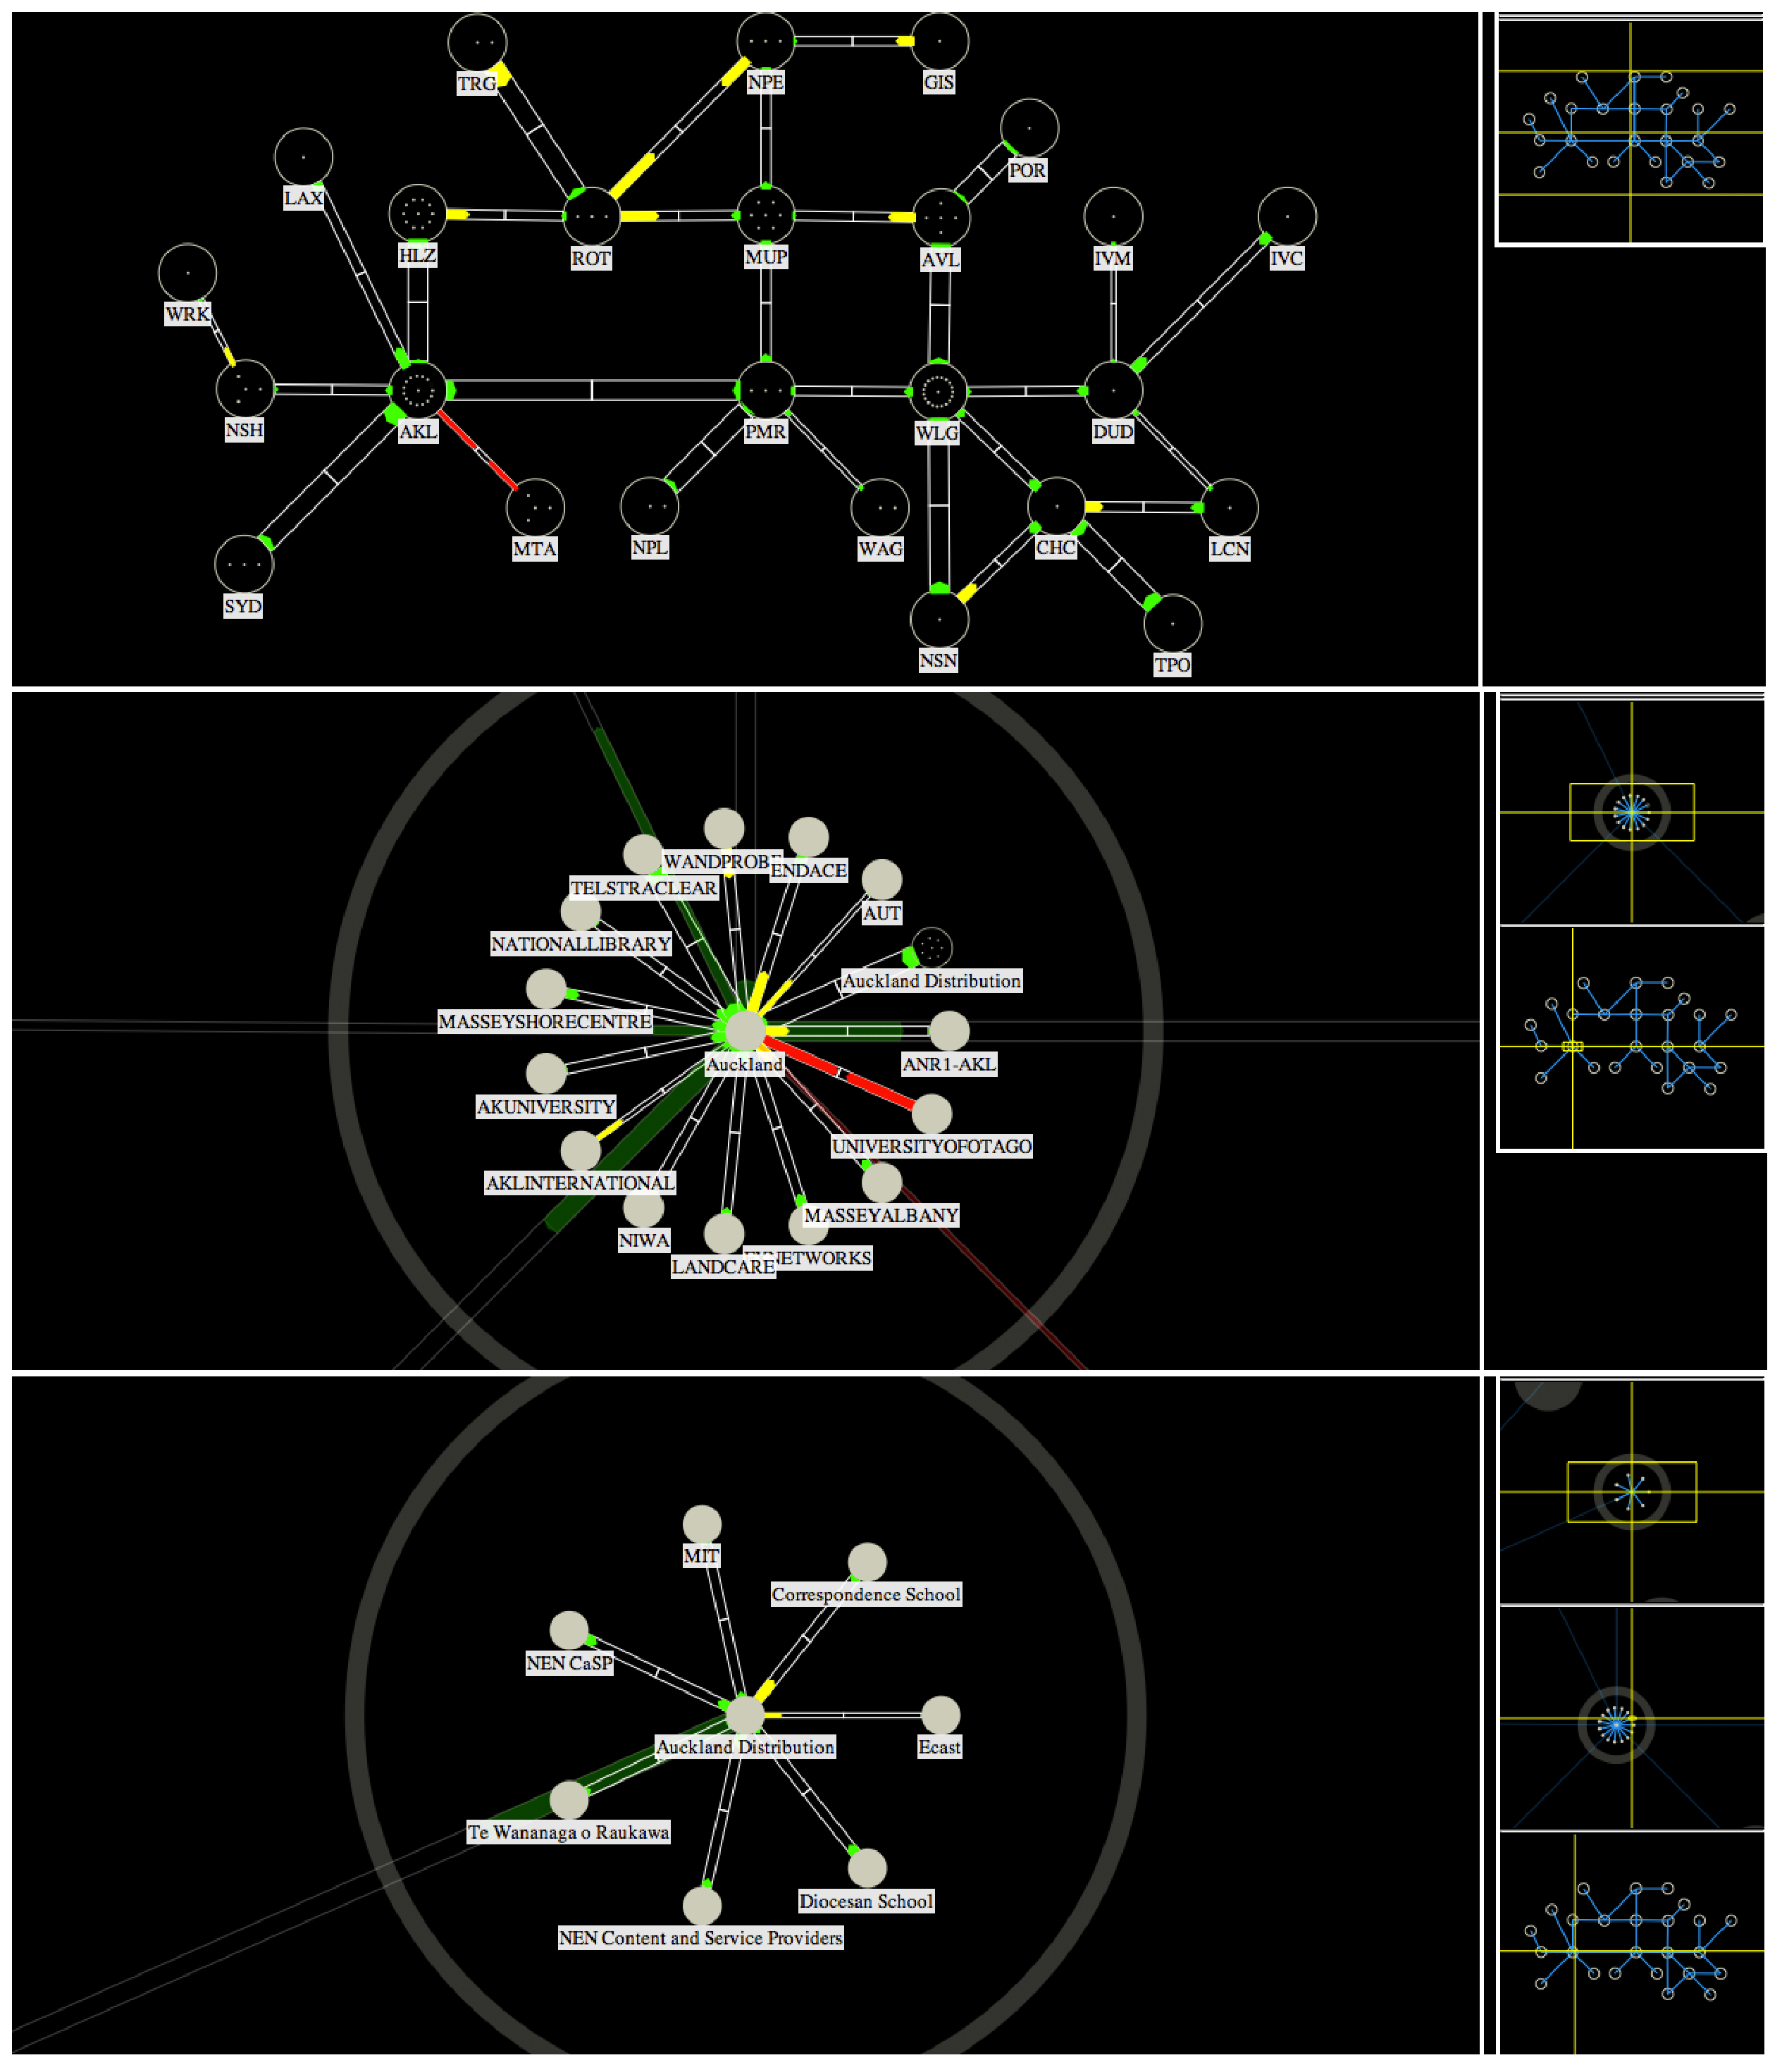
\includegraphics[width=170mm,height=197.95mm]{assets/overviews1-0.eps}
\caption{}
\label{fig:overviews1.0}
\end{figure}

\section{Implementation} 
\label{sec:implementation}
  % Overall implementation
  % Client side / server side
  %   * Polling performance data
  %   * Interact with user to request more server side data
  %   * Or just change visualisation parameters

\subsection{Nodes and Edges}
\label{sec:nodes-and-edges.impl}
  % How were nodes and edges implemented
  %   * Both have display method and contains method
  %   * Display: ..., Contains: ...
  %   * People producing a view may implement their own functions
  %   * Pipe-edges are one of these.
  %     > How did I implement these
  %     > rotated rectangular pipes, broken up into two sections
  %     > with height proportional to total bandwidth, length ...

\subsection{Groups}
\label{sec:groups.impl}

\subsection{Layouts}
\label{sec:layouts.impl}
  % 
  % Basic overview of star layout (because I implemented it myself)
  % Overview of layout system interface
  %
  %


\subsubsection{Editor}
\label{sec:editor.impl}

\subsection{Navigation}
\label{sec:navigation.impl}
  
  % Pan and Zoom + Space Scale diagrams - Space–scale Diagrams:Understanding Multiscale Interfaces
  % Pans are linear, zoom is logarithmic

\subsection{Overviews}
\label{sec:overviews.impl}

\subsection{Overlays}
\label{sec:overlays.impl}

\section{Deployment Examples}
\label{sec:deployment-examples}

\section{Evaluation}
\label{sec:evaluation}

\section{Future Work}
\label{sec:future-work}
  % Discuss possible branches of future work
  %   > Incorporate the map as part of a network management system
  %   > Experiment with more layout algorithms
  %   > Look into the posibility of effectively incorporating layers
  %   > Generate adapters to take common network data types such as RRD

\section{Conclusion}
\label{sec:conclusion}

%\bibliographystyle{plain}
%\bibliography{520-report}

\appendix
\appendixpage

\section{Karen PHP Network Weathermap}
\label{app:karenphp}
\centering
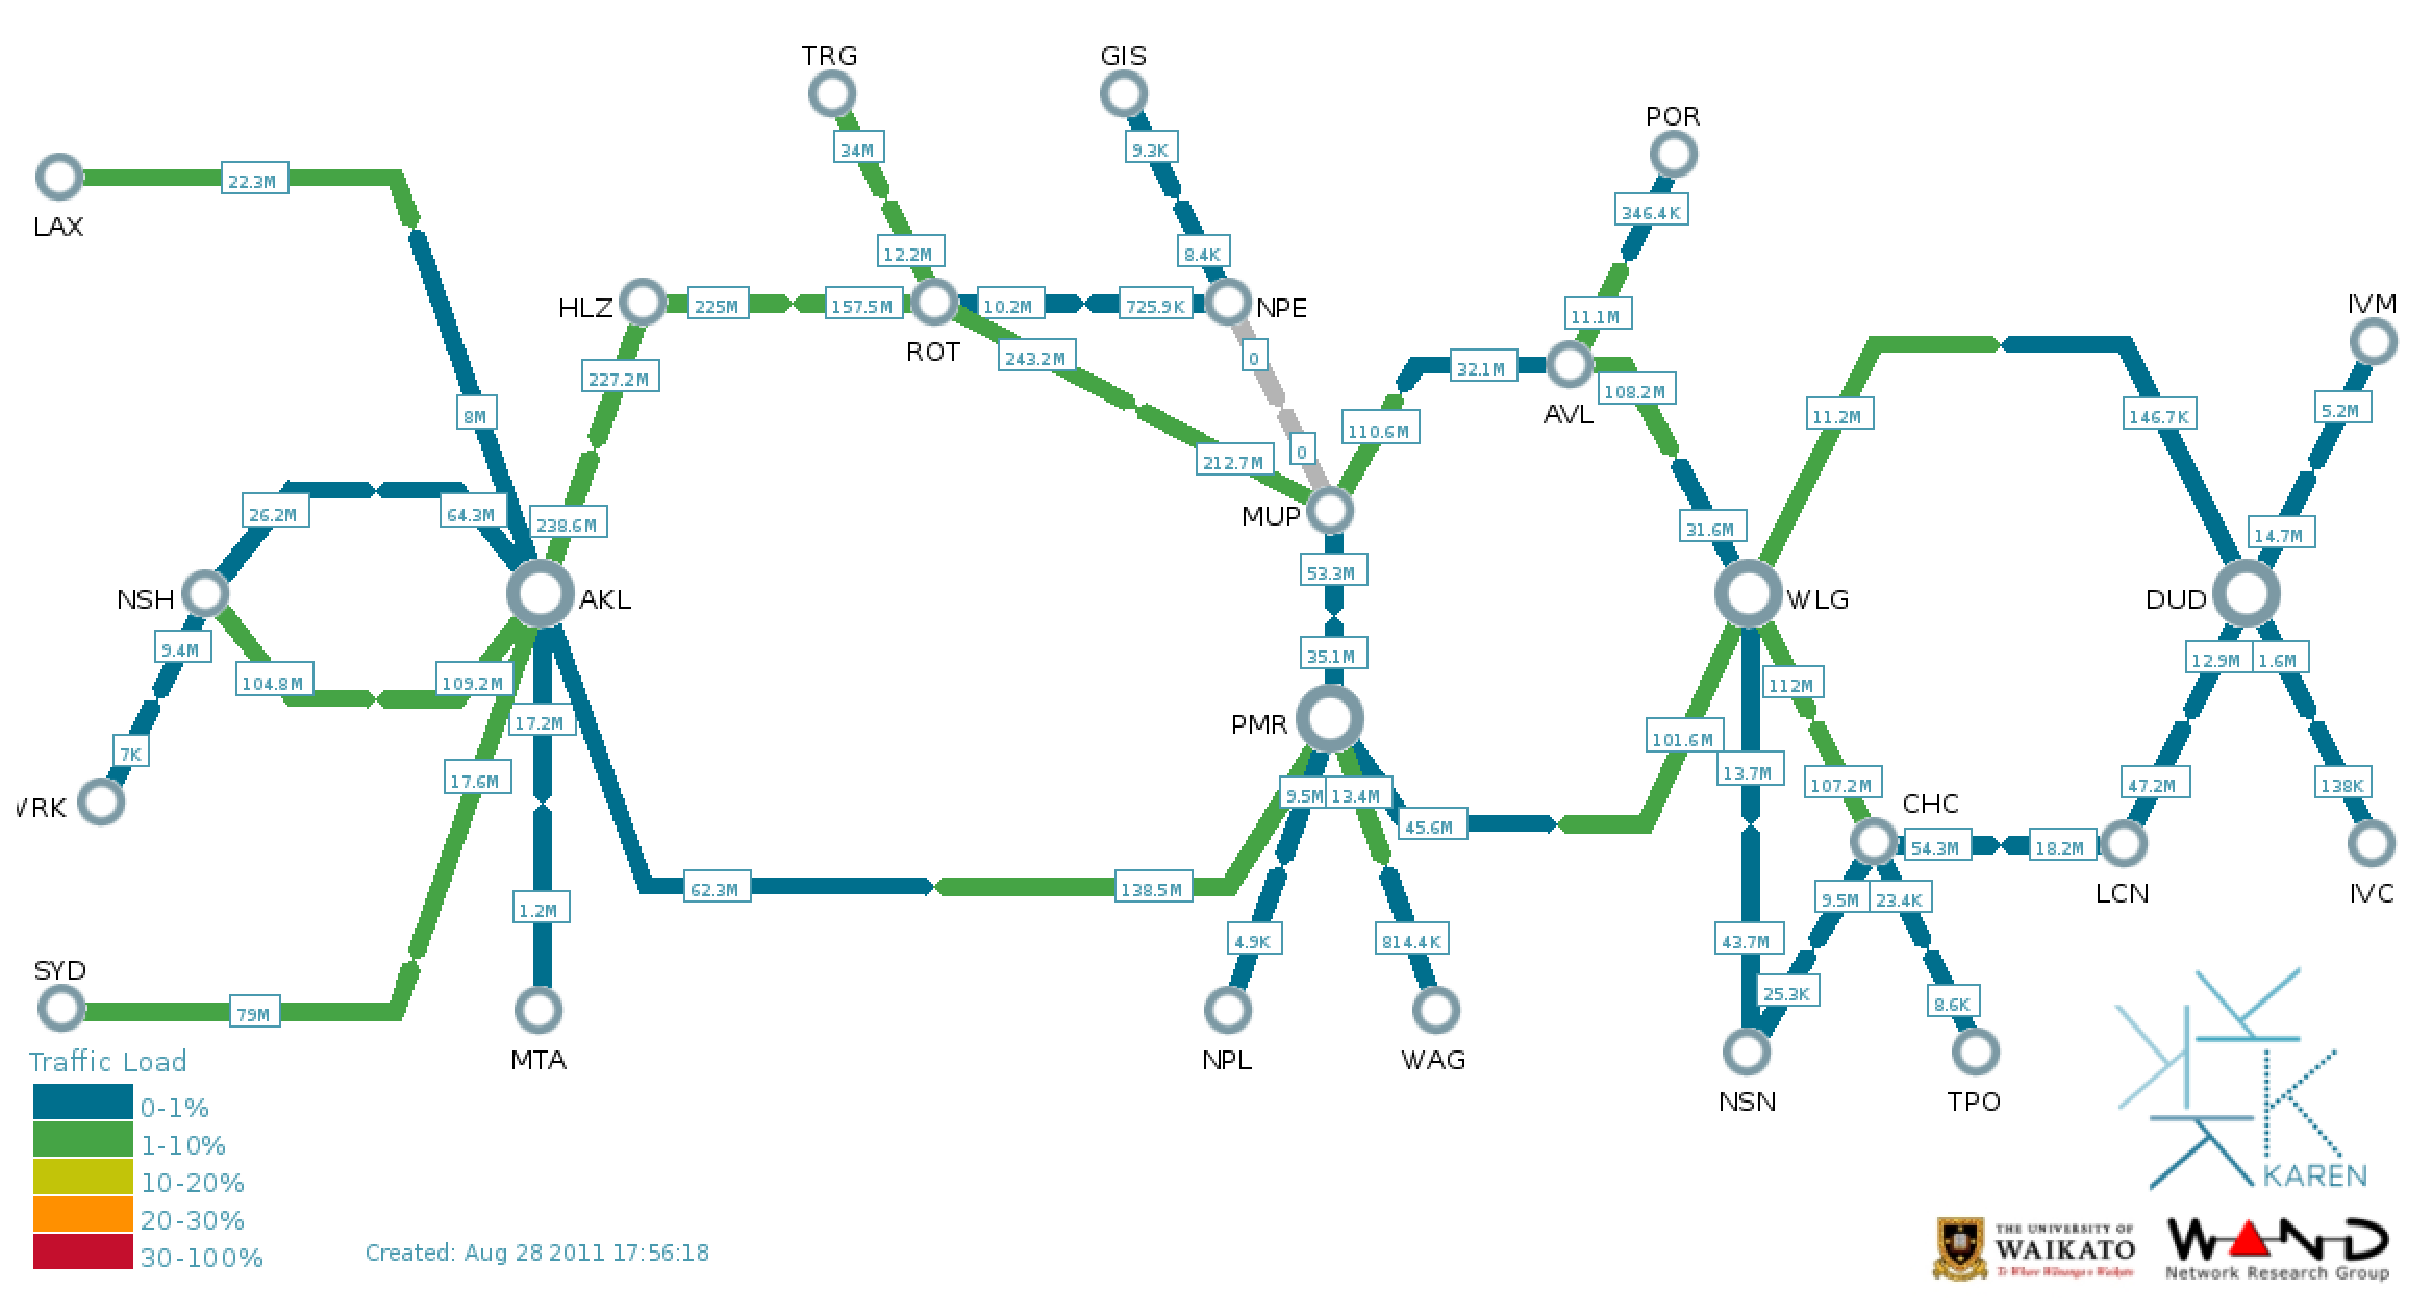
\includegraphics[width=170mm,height=90.76mm]{assets/karen-phpweathermap.eps}

\section{Rural Link Nagios Network Map}
\label{app:crcnetnagios}
\centering
\includegraphics[width=170mm,height=136mm]{assets/rurallink-nagios.eps}

\end{document}
